\documentclass[a4paper,12pt,oneside]{book}
\usepackage{graphicx}
\usepackage{fancyhdr}
\usepackage[font = scriptsize, bf]{caption}
\usepackage[italian]{babel}
\usepackage[utf8x]{inputenc}
\usepackage[parfill]{parskip}
\usepackage{amsmath, amssymb}
\usepackage{moreverb}
%\usepackage{subfig}
\usepackage{algorithm}
\usepackage{algpseudocode}
\usepackage[usenames,dvipsnames]{color}
\usepackage[swapnames]{frontespizio}
\usepackage{url}
\usepackage{setspace}
\usepackage{eqparbox,array}
\usepackage{siunitx}
\usepackage{subfigure} 
\usepackage{wrapfig}

\renewcommand{\algorithmiccomment}[1]{  //\emph{\textcolor{Gray}{#1}}}


% Sistema i margini per lasciare pi� spazio nella zona di rilegatura
\addtolength{\oddsidemargin}{+1,0cm} 
\addtolength{\evensidemargin}{+1,0cm} 
\onehalfspacing

% Imposta lo stile della prima pagina del capitolo
\fancypagestyle{plain}
{
    \fancyhead{}
    \fancyfoot[LE,RO]{\thepage}
    \renewcommand{\headrulewidth}{0pt}
}

\DeclareMathOperator*{\argmax}{arg\,max}
\newcommand{\compInterfacciaDB}{Data Interface}
\newcommand{\compLoader}{Loader}
\newcommand{\compMatrix}{Matrix Creator}
\newcommand{\compTermsSel}{Terms Selector}
\newcommand{\compPosition}{Position Calculator}
\newcommand{\compClustering}{Clustering Component}
\newcommand{\compEvolution}{Evolution Discoverer}

\hyphenation{ti-me-win-dow}

\graphicspath{{./Immagini/}}


\begin{document}
% Imposta lo stile di intestazione e pi� di pagina della parte iniziale
	% frontespizio
	\begin{frontespizio}
		\Universita{Bari - ``Aldo Moro''}
		\Logo[3.5cm]{logo_uni}
		\Divisione{Facolt� di Informatica}
		\Corso{\\Informatica e Tecnologie per la Produzione del Software}
		\Annoaccademico{2014-2015}
		\Titoletto{Tesi di laurea\\in\\Programmazione II}
		\Titolo{Url2Vec:\\Clustering di pagine in un grafo Web}
		\Candidato[587662]{Christopher Piemonte}
		\NCandidato{Laureando}
		\Relatore{Chiar.mo Prof. Michelangelo Ceci}
		\Relatore{Chiar.mo Prof. Donato Malerba}
		\Correlatore{Dott.ssa Pasqua Fabiana Lanotte}
		\Margini{3cm}{2cm}{2cm}{2cm}
	\end{frontespizio}
	
	\pagestyle{fancy}
	\fancyfoot{}
	\fancyfoot[LE,RO]{\thepage}
	\fancyhead{}
	\renewcommand{\headrulewidth}{0pt}
	\headheight = 15pt
	\frontmatter
	
	% dedica
	\null\vspace{\stretch{1}}
		\begin{flushright}
			\emph{Ai miei genitori ...}
		\end{flushright}
	\vspace{\stretch{2}}\null
	
	% indice
	\tableofcontents
	\listoftables
	\listoffigures
	\newpage
	\color{white}
	a
	\color{black}
%******************************************************************
% Materiale iniziale
%******************************************************************
%% !TEX encoding = UTF-8
% !TEX TS-program = pdflatex
% !TEX root = ../Tesi.tex
% !TEX spellcheck = it-IT

%*******************************************************
% Frontespizio
%*******************************************************
\begin{frontespizio}
\Preambolo{\usepackage{iwona}} % riga da commentare se non si carica ArsClassica

\Universita{Bologna}
\Logo{Sigillo}
\Facolta{Teologia}
\Corso{Belle Lettere}
\Annoaccademico{2011--2012}
\Titoletto{Tesi di laurea magistrale}
\Titolo{La mia tesi: \\ la prova ontologica \\ dell'esistenza di Dio}
\Sottotitolo{Alcune considerazioni mutevoli}
\Candidato[AB123456]{Lorenzo Pantieri}
\Relatore{Enrico Gregorio}
\Relatore{Claudio Beccari}
\Correlatore{Tommaso Gordini}
\Correlatore{Ivan Valbusa}
\end{frontespizio}





%*******************************************************
% Frontespizio alternativo
%*******************************************************
%\begin{titlepage}
%\pdfbookmark{Frontespizio}{Frontespizio}
%\changetext{}{}{}{((\paperwidth - \textwidth) / 2) - \oddsidemargin - \hoffset - 1in}{}
%\null\vfill
%\begin{center}
%\large
%\sffamily
%\bigskip

%{\LARGE\myName} \\

%\bigskip

%{\Huge\myTitle \\
%}

%\bigskip
    
%\vspace{9cm}

%\begin{tabular}{cc}
%\parbox{0.3\textwidth}{
\includegraphics[width=2.5cm]{Sigillo}}
%&
%\parbox{0.7\textwidth}{{\Large\myDegree} \\ 

%					{\normalsize
%					Relatore: \myProf \\
%%					Co-relatore: \myOtherProf \\
%					
%					\myUni \\
%					\myFaculty \\
%					\myDepartment \\
%					\myTime}}
%			\end{tabular}
%\end{center}
%\vfill
%\end{titlepage}







%% !TEX encoding = UTF-8
% !TEX TS-program = pdflatex
% !TEX root = ../Tesi.tex
% !TEX spellcheck = it-IT

%*******************************************************
% Colophon
%*******************************************************
\clearpage
\phantomsection
\thispagestyle{empty}

\hfill

\vfill

%\noindent\myName: \textit{\myTitle,}
%\myDegree,
%\textcopyright\ \MakeTextLowercase{\myTime}.

\lipsum[2]
%% !TEX encoding = UTF-8
% !TEX TS-program = pdflatex
% !TEX root = ../Tesi.tex
% !TEX spellcheck = it-IT

%*******************************************************
% Dedica
%*******************************************************
\cleardoublepage
\phantomsection
\thispagestyle{empty}
\pdfbookmark{Dedica}{Dedica}

\vspace*{3cm}

\begin{center}
Lorem ipsum dolor sit amet, consectetuer adipiscing elit. \\ \medskip
--- Oscar Wilde    
\end{center}

\medskip

\begin{center}
Dedicato a tutti gli appassionati di \LaTeX.
\end{center}
%% !TEX encoding = UTF-8
% !TEX TS-program = pdflatex
% !TEX root = ../Tesi.tex
% !TEX spellcheck = it-IT

%*******************************************************
% Indici
%*******************************************************
\cleardoublepage
\pdfbookmark{\contentsname}{tableofcontents}
\setcounter{tocdepth}{2}
\tableofcontents
\markboth{\spacedlowsmallcaps{\contentsname}}{\spacedlowsmallcaps{\contentsname}} 
\clearpage

\begingroup 
    \let\clearpage\relax
    \let\cleardoublepage\relax
    \let\cleardoublepage\relax
    %*******************************************************
    % Elenco delle figure
    %*******************************************************    
    \phantomsection
    \pdfbookmark{\listfigurename}{lof}
    \listoffigures

    \vspace*{8ex}

    %*******************************************************
    % Elenco delle tabelle
    %*******************************************************
    \phantomsection
    \pdfbookmark{\listtablename}{lot}
    \listoftables
        
    \vspace*{8ex}
       
\endgroup

\cleardoublepage

%% !TEX encoding = UTF-8
% !TEX TS-program = pdflatex
% !TEX root = ../Tesi.tex
% !TEX spellcheck = it-IT

%*******************************************************
% Sommario+Abstract
%*******************************************************
\cleardoublepage
\phantomsection
\pdfbookmark{Sommario}{Sommario}
\begingroup
\let\clearpage\relax
\let\cleardoublepage\relax
\let\cleardoublepage\relax

\chapter*{Sommario}

\lipsum[1]

\vfill

\selectlanguage{english}
\pdfbookmark{Abstract}{Abstract}
\chapter*{Abstract}

\lipsum[2]

\selectlanguage{italian}

\endgroup			

\vfill


%% !TEX encoding = UTF-8
% !TEX TS-program = pdflatex
% !TEX root = ../Tesi.tex
% !TEX spellcheck = it-IT

%*******************************************************
% Ringraziamenti
%*******************************************************
\cleardoublepage
\phantomsection
\pdfbookmark{Ringraziamenti}{ringraziamenti}

\begin{flushright}{\slshape    
	Lorem ipsum dolor sit amet, consectetuer adipiscing elit. \\
	Ut purus elit, vestibulum ut, placerat ac, adipiscing vitae, felis. \\
	Curabitur dictum gravida mauris.} \\ \medskip
    --- Donald Ervin Knuth
\end{flushright}


\bigskip

\begingroup
\let\clearpage\relax
\let\cleardoublepage\relax
\let\cleardoublepage\relax

\chapter*{Ringraziamenti}

\lipsum[1]

\bigskip
 
\noindent\textit{\myLocation, \MakeTextLowercase{\myTime}}
\hfill L.~P.

\endgroup
% !TEX encoding = UTF-8
% !TEX TS-program = pdflatex
% !TEX root = ../Tesi.tex
% !TEX spellcheck = it-IT

%*******************************************************
% Introduzione
%*******************************************************
\cleardoublepage
\chapter*{Introduzione}

La principale caratteristica dell'Era dell'Informazione è rappresentata dalla possibilità di generare, memorizzare, trasmettere e processare enormi quantità di dati in modo rapido ed economico.

 La disponibilità di una simile quantità di dati, elaborabili automaticamente, ha consentito un forte incremento del processo di generazione e diffusione di conoscenza, utilizzabile per migliorare processi decisionali. Ad oggi, tuttavia, tali risorse non sono appieno sfruttate in tutti i campi e il loro valore potenziale riserva ancora numerose sorprese.

Questo problema è particolarmente sentito nel contesto Web. Il Web infatti può essere considerato la più grande, eterogenea e dinamica sorgente informativa pubblicamente accessibile. Tali caratteristiche rendono il processo di analisi dei dati e estrazione di nuova conoscenza un task altamente complesso e apre nuove sfide e frontiere per l'Informatica.
%L'analisi di dati pubblicamente accessibili nel Web, l'estrazione di pattern e l'utilizzo degli stessi al fine di generare nuova conoscenza definiscono nuove sfide e frontiere per l'Informatica. 
%  La ricerca di pattern nella generazione e nell'utilizzo di nuovi contenuti web e la conoscenza che portano è un'area ancora giovane nell'informatica e in rapida crescita. 
%Con l'aumentare dei dati disponibili sul web e le potenzialmente infinite pagine generate dinamicamente, il bisogno di preprocessare questa informazione sembra scontrarsi con problemi computazionali. Indicizzare o cercare milioni di documenti non-omogenee sul web è diventata una sfida.

%Ogni giorno migliaia di utenti utilizzano il Web per acquisire informazioni ricercando informazioni su motori di ricerca o navigando siti web. Tuttavia, quelle peculiarità che contraddistinguono il Web come dimensione, eterogeneicità e dinamicità generano notevoli difficoltà per gli utenti nel modo di interagire, ricercare ed utilizzare le informazioni.

Un'importante sfida è rappresentata dal problema di organizzare i contenuti e la struttura dei documenti web.
%A dispetto della diversità delle pagine web nella rete, quelle che risiedono all'interno di una particolare organizzazione, spesso, condividono una certa struttura.
In particolare diversi lavori si sono concentrati sul problema del Web Clustering, ossia il processo di raggruppare pagine web in \textit{cluster} cosìcche ogetti simili  possano essere raggruppati nella stessa classe e oggetti dissimili possano essere raggruppati in classi differenti.
Gli obiettivi di questo processo possono essere molteplici: migliorare l'accessibilità alle informazioni e il ritrovamento delle stesse, comprendere i comportamenti di navigazione degli utenti, comprendere come le informazioni si distribuiscono su più pagine web, etc.

In quest'ottica nasce Url2vec, un sistema per il clustering di pagine web che utilizza il contenuto testuale delle pagine web e la struttura ad hyperlink del sito a cui le pagine da raggruppare appartengono, per estrarre cluster di pagine dello stesso tipo semantico (per esempio pagine web di professori, corsi, prodotti, etc.).

Differentemente dagli algoritmi di clustering di pagine web esistenti in letteratura, Url2Vec non considera un sito web come una collezione di documenti testuali indipendenti tra loro, ma cerca di combinare informazioni relative al contenuto con informazioni strutturali, in modo che due pagine web vengano considerate simili se  caratterizzate da una simile distribuzione di termini e abbiano una una simile correlazione nascosta all'interno dei cammini percorribili nel sito web.
%Il clustering di pagine web è un argomento trattato estensivamente in letteratura come un modo di raggruppare pagine  all'interno di cluster omogenei, anche se gran parte del lavoro svolto si basa su un insieme arbitrario di pagine derivanti da molteplici siti differenti. Relativamente poco è stato il lavoro svolto sul clustering di un specifico sito di una determinata organizzazione.
 
 %Infatti, Url2vec combinando e adattando tecniche di Data Mining e di Natural Language Processing, si propone come valida opzione per il clustering di pagine web estraendo informazioni latenti nella struttura degli hyperlink, denotando una correlazione nascosta nei cammini percorribili nel grafo del web.

Le motivazioni alla base dell'implementazione di Url2vec sono state guidate dal voler sfruttare conoscenza già immagazzinata nella risoluzione di problemi specifici in contesti differenti per il quale erano stati ideati, ricavando un trasferimento della conoscenza.
Infatti Url2Vec combina algoritmi tipici dell'area del Natural Language Processing con quelli della Teoria dei Grafi al fine di utilizzare in modo innovativo algoritmi estenti nel contesto Web. 
%L'obiettivo in particolare di questa tesi è estendere lo stato attuale esistente, implementando componenti per realizzare l'estrazione di pagine web correlate e raggrupparle sulla base delle sequenze attraversabili per vistarle, offrendo un diverso punto di vista considerando maggiormente le relazioni invece che il solo contenuto.

Si definisce di seguito la struttura di questo lavoro di tesi.\\
Nel capitolo 1 ci si occuperà di descrivere lo stato attuale, elencando le metodologie utilizzate, e di analizzare nel dettaglio le diverse problematiche da affrontare durante l'analisi dei dati.
Nel capitolo 2 saranno presentati gli obiettivi principali che la metodologia presentata ed il sistema realizzato hanno seguito, descrivendo nel dettaglio le diverse tecniche utilizzate per la realizzazione delle fasi necessarie all'individuazione dei pattern latenti nella struttura del web.
Nel capitolo 3 si parlerà della frontiera attuale dell'Informatica in tali campi confrontando similitudini e spunti di riflessione.
Nel capitolo 4 si descriverà la sperimentazione effettuata,completa di tabelle, grafici e commenti che evidenziano punti di forza e di debolezza individuati per ciascuna delle tecniche utilizzate per le diverse fasi eseguite dal sistema. Soffermandosi sulle novità introdotte con le metodologie presentate e cercando di confrontarle con quelle consolidate.
Infine nel capitolo 5 si parlerà dei possibili miglioramenti alle tecniche ed alle metodologie proposte.



%\pagestyle{scrheadings} 
%\cleardoublepage
%******************************************************************
% Materiale principale
%******************************************************************


% capitoli
	% frontespizio
	
	\frontmatter	
	\mainmatter

	% Imposta lo stile di intestazione e pi� di pagina dei capitoli
	\fancyfoot{}
	\fancyhead{}
	\fancyhead[LE,RO]{\slshape \leftmark}
	\fancyfoot[LE,RO]{\thepage}
	\renewcommand{\headrulewidth}{1pt}
	\renewcommand{\chaptermark}[1]{%
	\markboth{\thechapter.\ #1}{}}


\chapter{Informazioni latenti nel Web}
\label{cap:capitolo1}
% !TEX encoding = UTF-8
% !TEX TS-program = pdflatex
% !TEX root = ../Tesi.tex
% !TEX spellcheck = it-IT

%************************************************

%************************************************

Il progressivo aumento della dimensione del web e le informazioni in esso contenute fanno di esso il più grande insieme di dati da cui poter estrarre informazione velocemente e liberamente. Il Web è la sorgente informativa più eterogenea tra quelle esistenti, data la sua natura, e contenente dati prevalentemente non strutturati o semi-strutturati. Il problema non è sapere se le informazioni ci sono, ma riuscire a trovarle. Infatti anche se a prima vista il web sembra un insieme disordinato di pagine senza nessuna correlazione logica nella struttura, sia interna che nelle relazioni tra queste, in realtà possono essere trovate numerose correlazioni  nascoste. Riuscire ad estrarre informazione da questa enorme mole di dati può rivelare pattern molto specifici ed utilizzabili in numerose attività per produrre vantaggi competitivi. Recenti sviluppi nell'ambito di svariate aree dell'informatica hanno portato negli ultimi anni alla creazione di sempre più nuove ed efficaci tecniche. 
\\\\
Di seguito sarà introdotto il contesto del sistema, le varie aree in cui si colloca e da cui attinge le metodologie ed il bagaglio di conoscenza.
\section{Data Mining nel Web}
Il Data Mining è l'insieme di tecniche e metodologie che hanno per oggetto estrazione di informazione utile, di un sapere o di una conoscenza a partire da grandi quantità di dati.
\\
Tra le fasi più soggette a cambiamento al variare del dominio applicativo:
\begin{itemize}
\item estrazione di informazione implicita e nascosta da dati strutturati per renderla disponibile e direttamente utilizzabile; 
\item esplorazione ed analisi, eseguita in modo automatico o semiautomatico, su grandi quantità di dati allo scopo di scoprire pattern significativi.
\end{itemize}

In entrambi i casi i concetti di informazione e di significato sono legati strettamente al contesto in cui si esegue data mining, in altre parole un dato può essere interessante o trascurabile a seconda del tipo di applicazione in cui si vuole operare.
\\\\
Il \textbf{Web Mining} è l’applicazione delle tecniche di Data Mining per la scoperta e l’estrazione di conoscenza o di pattern dal World Wide Web.
Il web mining può essere diviso in tre principali categorie:
\begin{itemize}
\item \textit{Web Usage Mining} è l’applicazione di tecniche di Data Mining per la scoperta di pattern e informazioni utili attraverso l'analisi di log immagazzinati dai web server e contenenti click stream. 
Obiettivo di questo campo è l'apprendimento dell'identità, origine e comportamenti degli utenti che navigano i siti web al fine di comprendere i loro bisogni e ad offrire loro servizi migliori attraverso una personalizzazione dell'esperienza web.
\item \textit{Web Structure Mining} consiste nell'estrazione di relazioni sconosciute o nascoste tra pagine web attraverso l'analisi della struttura ad hyperlink di un sito web (anche chiamato ``grafo web''). Questo task verrà analizzato in dettaglio nella sezione \ref{subsec:webstructure}.
\item \textit{Web Content Mining} consiste nell'estrazione ed integrazione di informazione utile e precedentemente sconosciuta dal contenuto delle pagine web. Ricadono in questo campo due principali tipologie di algoritmi: \textit{i)} algoritmi capaci di raggruppare e classificare pagine web in funzione del loro contenuto testuale o del topic descritto; \textit{ii)} algoritmi per estrarre pattern significativi all'interno del contenuto delle pagine web (per esempio liste di prodotti commerciali, professori, etc.).  
Sebbene questi algoritmi possano sembrare molto simili ai più famosi algoritmi di Data Mining e Text Mining, le pagine web hanno delle proprietà e peculiarità che rendono tali algoritmi non direttamente applicabili. Un'importante branca del Web Content Mining è rappresentato dal Web Information Extraction, il cui obiettivo è quello di estrarre dati strutturati da pagine web e integrarli in tabelle relazionali. In questo contesto il Web Content Mining può essere visto quindi come reperimento e immagazzinamento di informazioni.
\end{itemize}

Quando si confronta il web mining con il data mining tradizionale, ci sono tre principali differenze da considerare:
\begin{itemize}
\item \textbf{Scalabilità}:\color{red}cos'è la scalabilità?? mettere una definizione, piu formale
\color{black}
 Nel data mining tradizionale, processare un milione di record può essere considerato sopra la media, mentre nel web mining dieci milioni di pagine possono non essere abbastanza.
\item \textbf{Accesso}: Quando si analizzano informazioni aziendali, i dati sono privati e spesso richiedono diritti di accesso per la lettura. Nel web mining i dati sono pubblici e non richiedono alcun tipo di permesso, anche se a volte il crawling deve essere effettuato secondo determinate politiche, cercando di non sovraccaricare il sito effettuando numerose richieste.
\item \textbf{Struttura}: I tradizionali task di data mining estraggono informazioni da un database, che assicura un certo livello di strutturazione dei dati. Task di web mining invece elaborano dati non strutturati o semi-strutturati. Anche quando le informazioni provengono da un database, la struttura è spesso coperta da tag HTML.
\end{itemize}
\color{red}
INSERIRE INFORMAZIONI CARATTERISTICHE DEL WEB (DIMENSIONE, DINAMICITA...SOCIETA VIRTUALE, PAG 5-7) IN MODO DA COLLEGARE IL CONCETTO DELL'ESISTENZA DI DATI STRUTTURATI E NON STRUTTURATI
\color{black}
\\
Enormi sforzi son stati fatti per combinare informazione strutturata e non strutturata presente all'interno di pagine web, al fine di estrarre, indicizzare e reperire nuova conoscenza. 
La maggior parte delle soluzioni attuali trasformano il contenuto testuale delle pagine web in uno spazio vettoriale \cite{}\color{red}https://www.jair.org/media/2934/live-2934-4846-jair.pdf \color{black}. Modelli basati su spazi vettoriali sono fondamentali per task che coinvolgono il calcolo della similarità tra oggetti in cui oggetti simili sono caratterizzati da rappresentazioni vettoriali simili. Il modello vettoriale \textit{termini-documenti} rappresenta il più semplice e utilizzato modello di rappresentazione di documenti testuali nel contesto del Text Mining. In tale modello il valore dell'elemento $i$-esimo in un vettore documento rappresenta il numero di volte che il termine $i$ compare nel documento stesso.    
Gli algoritmi basati su modelli di rappresentazione vettoriali si basano sull'assunzione di indipendenza tra i termini all'interno di un documento e tra i documenti stessi. Le pagine web violano come tutti i documenti testuali la prima assunzione, inoltre i collegamenti ipertestuali definendo relazioni di interdipendenza tra le pagine stesse comportano la violazione della seconda assunzione.

Di conseguenza gli algoritmi di Web Mining devono tener conto delle informazioni relative alla struttura del sito web a cui appartengono al fine di estrarre informazioni più accurate.

\section{Web Structure mining}
\label{subsec:webstructure}
Un enorme quantità di informazioni dal web sono rappresentati come dati semi-strutturati, ossia come combinazione di testo non strutturato e dati strutturati. I dati strutturati contenuti nelle pagine web sono tipicamente dati generati dinamicamente dalla struttura sottostante, come un database relazionale, o da un template statico.
\\\\
Estrarre questi dati è utile in molti domini applicativi perchè permette di ottenere ed integrare dati da diverse fonti, producendo così servizi migliori, informazioni personalizzate, meta-ricerche. Con sempre più aziende ed organizzazioni che disseminano informazioni in rete, l’abilità di estrarre questi dati dalle pagine web sta diventando estremamente importante.
\\\\
Differentemente dai documenti testuali tradizionali, i dati strutturati nelle pagine web sono arricchiti da hyperlink che dividono l’informazione in molteplici ed interdipendenti pagine web. Questi hyperlink possono essere usati per identificare le entità provenienti dal mondo reale (e.g. pagine di professori, corsi, prodotti) e le relazioni che intercorrono fra di esse. Dato che i documenti web non sono nè strutturati come un database nè completamente non-strutturati come documenti testuali, le tecniche tradizionali di data mining o text mining non possono essere applicate direttamente. 
\\\\
Nel primo caso, le tecniche di data mining si basano sul presupposto che i dati usati per apprendere un modello condividono uno schema comune, avente delle tabelle ben definite con attributi, colonne, tuple e vincoli. Le pagine web non hanno questo presupposto perchè contengono dati eterogenei e gli hyperlink definiscono relazioni il cui significato può variare profondamente. Inoltre le pagine web sono codificate in HTML che, differentemente da altri linguaggi di markup, è stato progettato solo per la renderizzazione dei dati. Per questa ragione, il web può essere considerato un moderno legacy system, in quanto una grande quantità di dati non è facilmente accessibile e manipolabile direttamente. 
\\\\
Nel secondo caso, le tecniche di text mining falliscono nell’apprendere modelli accurati perchè richiedono collezioni di documenti scritti in modo consistente e non sono in grado di gestire informazioni complesse con elementi che possiedono diversi ruoli semantici e che forniscono diverse funzionalità. Infatti differentemente dai documenti testuali, le pagine web hanno molteplici rappresentazioni che forniscono differenti informazioni. Una è la rapresentazione testuale del testo HTML, l’altra è la rappresentazione visuale renderizzata da un web browser. Algoritmi di text mining si concentrano sulla rapresentazione testuale ed ignorano la rappresentazione visuale. Di conseguenza, esiste un forte bisogno nel campo dell’informatica di creare approcci e tecniche che usando informazioni testuali, strutturali e visuali sono capaci di estrarre uno schema da dati strutturati ed allineare i dati seguendo tale schema.
\\\\
Il Web Structure Mining può essere diviso in due tipi:
\begin{itemize}
\item Estrazione di dati strutturati tra pagine web attraverso l'analisi del sito web. In questo caso un sito web è rappresentato come un grafo $G = (V, E)$ dove $V$ è l'insieme delle pagine web e $E$ è l'insieme degli hyperlink.
\item Estrazione di dati strutturati contenuti in una pagina web, analizzandone la struttura ad albero basata su tag HTML ed XML.
\end{itemize}
Tra i più importanti algoritmi di web structure mining troviamo Page Rank\cite{} e HITS\cite{}, i quali sfruttano la struttura ad hyperlink del Web per estrarre rank di pagine web.

\section{Rappresentazioni vettoriali di pagine Web}
Poichè 
La carenza di struttura delle pagine web obbliga all'effettuare dei passaggi preliminari per rendere processabili i dati disponibili. Metodi efficaci consistono nel rappresentare le pagine web come vettori, motivato dal fatto che task di machine learning richiedono input che sono matematicamente e computazionalmente convenienti da elaborare, considerando solo un sottoinsieme significativo dei dati in modo da astrarre ed eliminare informazioni ritenute non pertinenti al risultato finale. Questa fase è probabilmente la più importante in quanto algoritmi di apprendimento tanto bene quanto meglio i vettori ricavati rappresentano bene i dati di partenza. È necessario quindi estrarre rappresentazioni utili dai dati grezzi. Esistono molti modi per ricavare questa correlazione, come reti neurali, matrici di co-occorrenza, dimensionality reduction o rappresentazioni del contesto in cui appare la parola. L'alternativa proposta in questa tesi consiste nell'utilizzare tecniche di word embedding per apprendere rappresentazioni utili.
Il word embedding è il nome di un insieme di tecniche per il language modeling e per il feature learning nel campo del Natural language processing (NLP)\cite{Bengio03}. Utilizzate  in collezioni di documenti dove ad ogni parola viene associato un vettore, detto feature vector. 
\\\\
\color{red}come sei arrivato da rappresentazione vettoriale a word embedding?\color{black}
Il word embedding può essere visto come una funzione parametrizzata 
\begin{equation}
  W : words \to \mathbb{R^n}
\end{equation}
che associa una parola in un dato linguaggio ad un vettore multidimensionale. Un esempio potrebbe essere:
\begin{equation}
  W\left ( "cat" \right ) = \left ( 0.2, -0.4, 0.7, \ldots \right )
\end{equation}
A parole simili corrisponde un vettore simile. Se si cambia una parola con un sinonimo, la validità della frase in esame non cambia (e.g. molti cantano bene $\to$ tanti cantano bene). Questo permette di generalizzare da una frase ad una classe di frasi simili o di capire se una frase è valida, ovvero se  è formulata correttamente.  
\\\\
Questo non significa solo poter scambiare una parola con un sinonimo, ma anche di cambiare una parola con una altra in una classe simile (eg. il muro è rosso → il muro è blu) \cite{Collobert11}. Questo può essere appreso analizzando il contesto della parola da analizzare. Ad esempio ci saranno molti casi in cui sono state osservate frasi valide di questo tipo, quindi cambiando la parola “rosso” con la parola “blu” porterebbe alla creazione una frase ugualmente valida. 
\begin{figure}[htb]
	\centering
	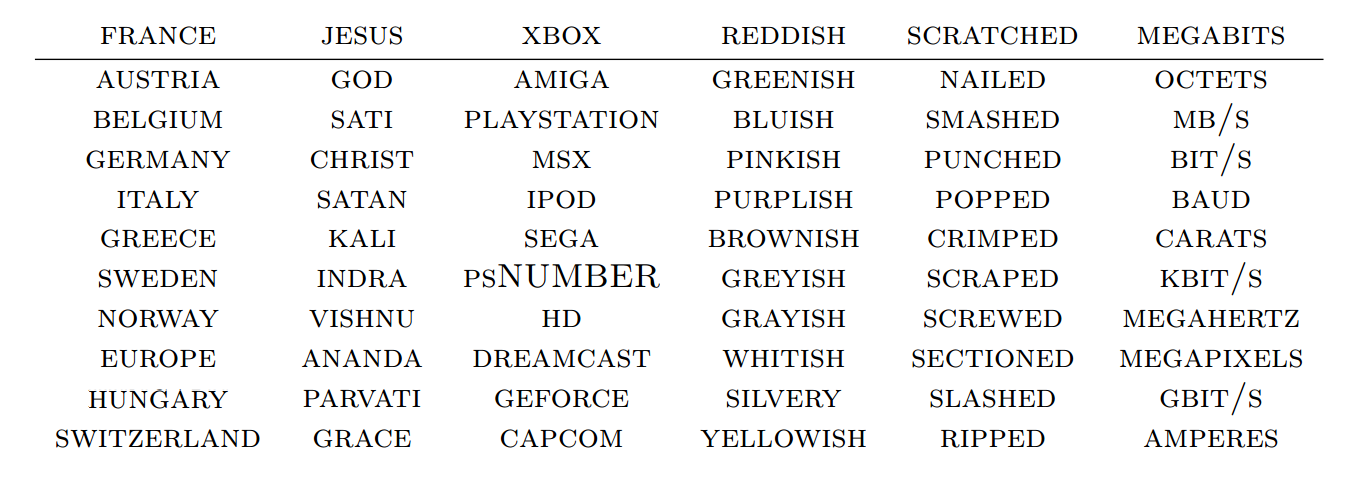
\includegraphics[width = 100mm]{weanalogies.png}
	\caption{Parole con vettori simili}
	\label{similarwords}
\end{figure}

Da questo potrebbe sembrare necessario osservare esempi relativi ad ogni parola per permetterci di generalizzarla. Comprendi tutte le parole che hai già visto, ma non hai già visto tutte le frasi che riesci a capire. Questo è l’approccio delle reti neurali.

\paragraph{Analogie}Il word embedding mostra un altra proprietà interessante anche se molto controversa: le analogie. Le analogie tra parole sembrano essere nascoste nella differenza dei loro rispettivi vettori \cite{Mikolov13}. 
\begin{equation}
  W\left ( "woman" \right ) -  W\left ( "man" \right ) \simeq W\left ( "aunt" \right ) -  W\left ( "uncle" \right )
\end{equation}
Da questo si evince che c’è una correlazione tra delle parole e le rispettive forme del genere opposto in quanto appariranno in contesti simile, differenti solo per alcuni dettagli come pronomi o articoli. Stessa cosa per tra singolare e plurale \cite{Mikolov13}.
\begin{figure}[htb]
	\centering
	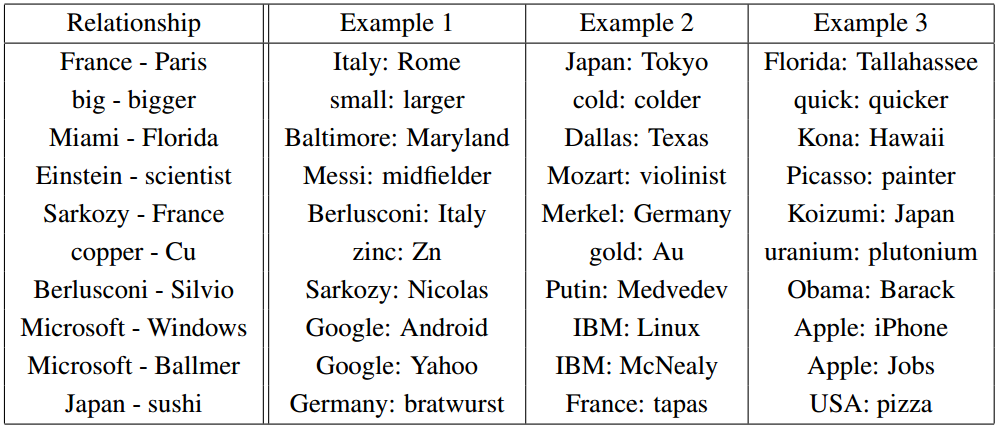
\includegraphics[width = 100mm]{weanalogies2.png}
	\caption{Alcuni esempi di analogie}
	\label{analogies}
\end{figure}
Queste proprietà possono essere considerate effetti collaterali. Non si è cercato di far apprendere il modello in modo da avere parole simili vicine fra loro. Questo sembra essere un punto di forza delle reti neurali nell’apprendere features che rappresentano bene i dati in modo automatico. invece di apprendere un rappresentazione dei dati specifica ed usarla per diversi task, è possibile apprendere un metodo per associare diversi tipi di dati in una singola rappresentazione. Queste tecniche sono note come transfer learning, metodi per applicare la conoscenza già appresa in contesti simili.
\\\\
Un esempio può essere il word embedding di parole linguaggi diversi. Dato che parole simili saranno associate a vettori simili, parole con significato simile in una lingua e nell’altra finiranno vicine tra loro, così come i loro sinonimi. È possibile notare che anche parole di cui non si conosceva la traduzione o che avessero significati simili, sono finite vicine tra loro \cite{Zou13}.
\begin{figure}[htb]
	\centering
	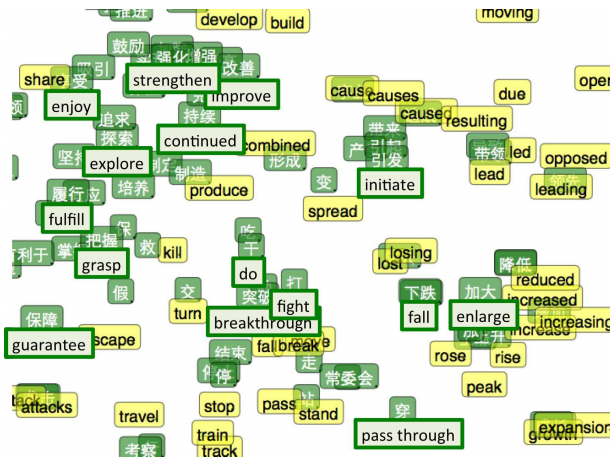
\includegraphics[width = 100mm]{englishchinese.png}
	\caption{Visualizzazione con t-SNE di un word embedding bilingua. }
	\label{englishchinese}
\end{figure}

\subsection{Word2vec}
\label{word2vec}
Un algoritmo molto famoso di word embedding è il recente word2vec. L’algoritmo usa i documenti per far apprendere una rete neurale, massimizzando la probabilità condizionata del contesto data una parola, applicando il modello appreso ad ogni parola per ricavare il vettore corrispondente e calcolando il vettore della frase facendo la media dei vettori delle parole, costruisce la matrice di similarità delle frasi ed usa PageRank per classificare le frasi nel grafo.
\begin{equation}
   arg\max_{\theta} \prod_{\left ( w, c \right ) \in D} p\left ( c|w; \theta \right )
\end{equation}
L’obiettivo è di ottimizzare il parametro $ \left (\theta \right )$ massimizzando la probabilità condizionata del contesto $\left ( c \right )$ data la parola $\left ( w \right )$. $D$ è l’insieme di tutte le coppie $\left ( w, c \right )$. 
Per esempio: “ho mangiato un \underline{\hspace{1cm}}  al McDonald ieri sera”, molto probabilmente restituirà “Big Mac”.
\\\\
Applicare il modello di ogni parola per ottenere il suo vettore corrispondente (Figura \ref{2w2v})
\begin{figure}[htb]
	\centering
	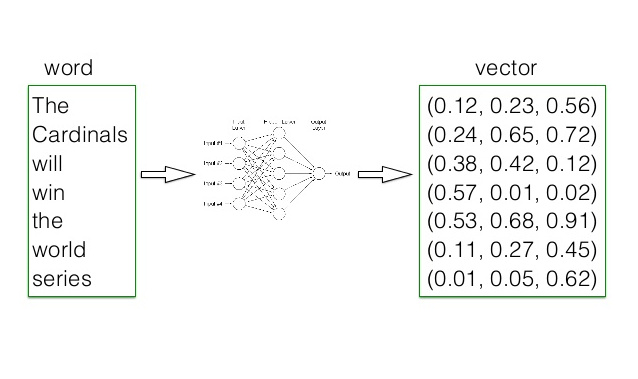
\includegraphics[width = 100mm]{2w2v.jpg}
	\caption{Vettori corrispondenti alle parole}
	\label{2w2v}
\end{figure}
\\\\
Calcolare il vettore delle frasi facendo la media del vettore delle loro parole (Figura \ref{3w2v})
\begin{figure}[htb]
	\centering
	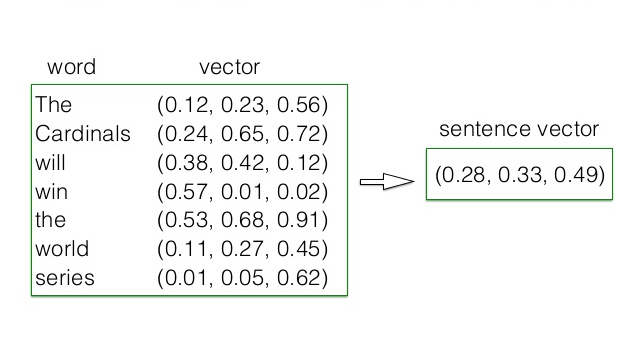
\includegraphics[width = 100mm]{3w2v.jpg}
	\caption{Vettori corrispondenti alle frasi}
	\label{3w2v}
\end{figure}
\\\\
Costruire la matrice di similarità delle frasi (Figura \ref{4w2v})
\begin{figure}[htb]
	\centering
	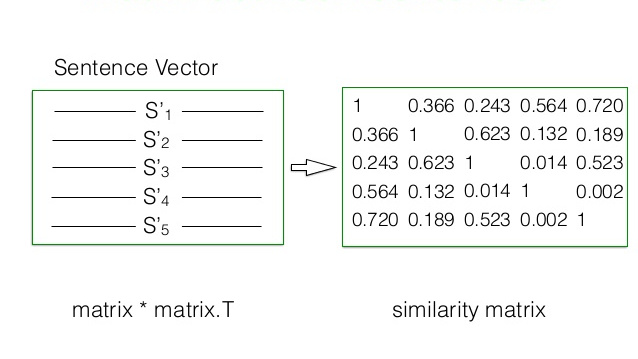
\includegraphics[width = 100mm]{4w2v.jpg}
	\caption{Matrice di similarità}
	\label{4w2v}
\end{figure}
\\\\
Infine usare PageRank par classificare le frasi nel grafo.
 (Figura \ref{5w2v})
\begin{figure}[htb]
	\centering
	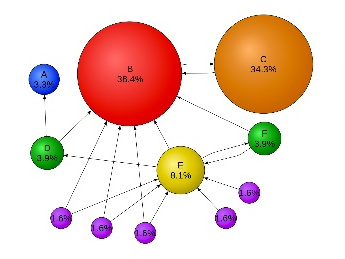
\includegraphics[width = 100mm]{5w2v.jpg}
	\caption{Assegna uno "score" utilizzando Pagerank}
	\label{5w2v}
\end{figure}

Word2vec è una rete neurale a due layer, sebbene non sia profonda (deep neural network) come spesso definita, trasforma il testo in modo che altre reti neurali possano comprenderlo. Prende in input un corpus di documenti e genera un insieme di vettori: feature vectors per ogni parola del corpus. I vettori restituiti sono rappresentazioni numeriche del contesto della singola parola. 
\\\\
Dati abbastanza dati, utilizzo e contesti, word2vec può apprendere rappresentazioni delle parole altamente accurate, basate sulle apparizioni della parola nei diversi contesti. Queste rappresentazioni possono essere usate per trovare associazioni fra parole o per raggruppare documenti e classificarli per argomento. La similarità fra i vettori può essere misurata attraverso la coseno similarità, dove nessuna similarità è espressa come un angolo di 90 gradi, mentre una similarità totale è data  da un angolo di 0 gradi tra i vettori. Ad esempio il vettore relativo a “Sweden” è uguale al vettore “Sweden” mentre il vettore “Norway” ha una distanza di similarità di $0.760124$.
\\\\
Word2vec può apprendere rappresentazioni principalemente in due modi, o usando il contesto per predire la parola data (metodo conosciuto come “continous bag of word”, o \textbf{CBOW}), o usando una parola per predire il contesto (\textbf{skip-gram}).

\section{Random Walk}
In matematica, un Random Walk è la formalizzazione dell'idea di prendere passi successivi in direzioni casuali. Matematicamente parlando, è il processo stocastico più semplice, il processo markoviano. Qui sono utilizzati per ricavare percorsi pseudo casuali da attraversamento del grafo del web per ottenere sequenze di URL collegati semanticamente.
\\\\
In una passeggiata aleatoria monodimensionale si studia il moto di una particella puntiforme vincolata a muoversi lungo una retta nelle due direzioni consentite. Ad ogni movimento essa si sposta (a caso) di un passo a destra (con una probabilità fissata $\ p$) o a sinistra con una probabilità $\ 1-p$, ed ogni passo è di lunghezza uguale e indipendente dagli altri.
\begin{figure}[htb]
	\centering
	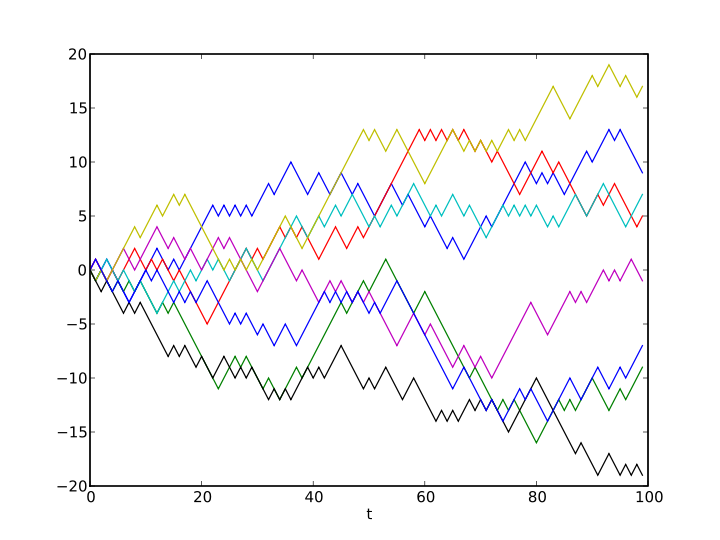
\includegraphics[width = 100mm]{randomwalkonedim.png}
	\caption{Rappresentazione visuale di 8 random walk monodimensionali. }
	\label{englishchinese}
\end{figure}
\\\\
In una passeggiata aleatoria bidimensionale si studia il moto di una particella vincolata a muoversi sul piano spostandosi casualmente ad ogni passo a destra o a sinistra con probabilità $\frac{1}{2}$, verso l'alto o verso il basso con probabilità $\ p=\frac{1}{2}$. In pratica ad ogni passo può compiere un movimento lungo una delle quattro diagonali con probabilità $\frac{1}{4}$. Ci si chiede con che probabilità la particella tornerà al punto di partenza.
\begin{figure}[htb]
	\centering
	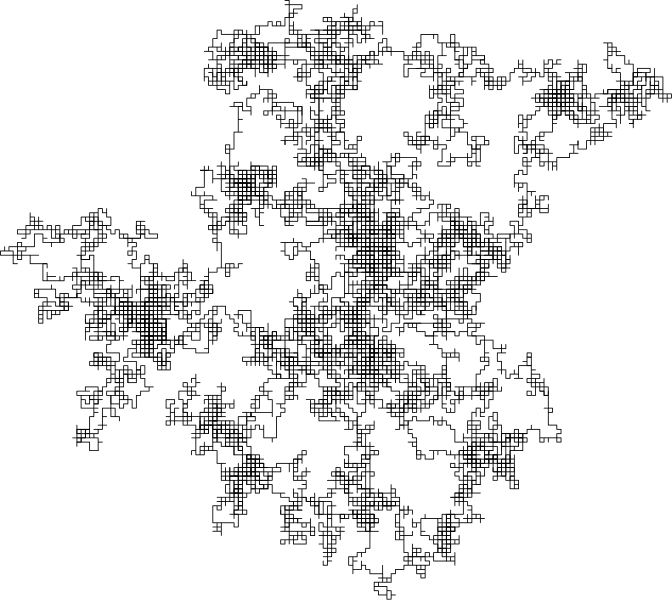
\includegraphics[width = 100mm]{randomwalktwodim.png}
	\caption{Rappresentazione visuale di un random walk di 25.000 passi su due dimensioni. }
	\label{englishchinese}
\end{figure}
\\\\
Queste passeggiate aleatorie possono trovare effettivi riscontri in natura come il traiettoria percorso da una particella in un liquido o in un gas, il tragitto di un animale affamato o anche il prezzo di un titolo fluttuante o la situazione finanziaria di un giocatore d'azzardo. Tutti questi esempi possono essere espressi come random walk, anche se in natura potrebbero non essere veramente casuali.
\\\\
Un popolare modello di random walk è quello su un reticolo regolare, dove ad ogni passo si segue un determinato percorso basandosi su una qualche distribuzione di probabilità. Nel caso più semplice si può solo “saltare” sul sito vicino. In un semplice random walk simmetrico in un reticolo localmente finito, le probabilità di saltare su ognuno dei siti vicini è la stessa.
\\\\
Per definire un random walk formalmente, prese indipendenti variabili casuali $ Z_1, Z_2, Z_3, $ \dots dove ogni variabile è o 1 o -1, con una probabilita del 50\% per ognuno dei due casi, e dato 
\begin{equation}
  S_0 = 0
\end{equation}
\begin{equation}
  S_n = \sum_{j=1}^{n} Z_j
\end{equation}
  
la serie $\left \{ S_n \right \} $ è chiamata random walk semplice in $\mathbb{Z}$.
\\\\
Si consideri un attraversatore casuale della rete (random surfer) che, partendo da un pagina web, esegue un passo alla volta in questo modo: ad ogni iterazione, dalla pagina corrente, procede verso una pagina a caso tale che esiste un link che dalla pagina corrente punta a questa.
\\\\
Procedendo da pagina a pagina, visiterò alcuni nodi, più spesso di altri; intuitivamente, saranno nodi con molti link entranti da altri nodi frequentemente visitati.
\\\\
Ci sono alcuni problemi. Che succede se si arriva ad una pagina che non ha link in uscita? In questo caso è necessario introdurre un’altra operazione: il teletrasporto. In questa operazione l’attraversatore casuale salta dal nodo corrente ad un qualsiasi altro nodo sulla rete.
Se $N$ è il numero totale dei nodi nel grafo, l’operazione di teletrasporto porta l’attraversatore verso ogni nodo con probabilità $\frac{1}{N}$. Potrebbe anche trasportarsi sulla posizione corrente con probabilità di $\frac{1}{N}$. Questa operazione è chiamata quando si arriva ad un non senza nodi in uscita o con una probabilità$\ d$ data, con$\ 0 < d < 1$.


\section{Clustering}
Sono un insieme di tecniche di analisi multivariata dei dati volte alla selezione e raggruppamento di elementi omogenei in un insieme di dati \cite{tryon}. Le tecniche di clustering si basano su misure relative alla somiglianza tra gli elementi. In molti approcci questa similarità (o dissimilarità) è concepita in termini di distanza in uno spazio multidimensionale. La bontà delle analisi ottenute dagli algoritmi di clustering dipende molto dalla scelta della metrica, e quindi da come è calcolata la distanza. Gli algoritmi di clustering raggruppano gli elementi sulla base della loro distanza reciproca, e quindi l'appartenenza o meno ad un insieme dipende da quanto l'elemento preso in esame è distante dall'insieme stesso dividendo gli elementi in più cluster(soft/fuzzy clustering) o in un solo cluster(hard cluster).
Le tecniche di clustering si possono basare principalmente su due "filosofie":
partizionale e gerarchico.

\subsubsection{Partizionale}
Gli algoritmi di clustering di questa famiglia creano una partizione delle osservazioni minimizzando una certa funzione di costo:
\begin{equation}
  \sum_{j=1}^{k} E\left ( C_j \right )
\end{equation}
dove $ k$ è il numero desiderato di cluster, $ C_j$ è il j-esimo cluster e $ E : C \to \mathbb{R^+}$ è la funzione di costo associata al singolo cluster. L'algoritmo più famoso appartenente a questa famiglia è il k-means, chiamato così da MacQueen nel 1967 \cite{MacQueen67}.

\subsubsection{Gerarchico}
Nel clustering gerarchico, invece, è necessario individuare il cluster da suddividere in due sottogruppi. Per questa ragione sono necessarie funzioni che misurino la compattezza del cluster, la densità o la distanza dei punti assegnati ad un cluster. Le funzioni normalmente utilizzate nel caso divisivo sono:
\paragraph{Single-link proximity}
Calcola la distanza tra i due cluster come la distanza minima tra elementi appartenenti a cluster diversi:
\begin{equation}
  D\left ( C_i, C_j \right ) = \min_{x \in C_i, y \in C_j} d\left ( x, y \right )
\end{equation}

\paragraph{Average-link proximity}
Questa funzione calcola la distanza tra i due cluster come la media delle distanze elementi:
\begin{equation}
  D\left ( C_i, C_j \right ) = \frac{1}{|C_i||C_j|}\sum_{x \in C_i, y \in C_j} d\left ( x, y \right )
\end{equation}

\paragraph{Complete-link proximity}
Questa funzione valuta la distanza massima tra due punti interni ad un cluster. Tale valore è noto anche come 'diametro del cluster': più tale valore è basso, più il cluster è compatto:
\begin{equation}
  D\left ( C_i, C_j \right ) = \max_{x \in C_i, y \in C_j} d\left ( x, y \right )
\end{equation}

\paragraph{Distanza tra centroidi}
Questa funzione valuta la distanza massima tra due punti interni ad un cluster. Tale valore è noto anche come 'diametro del cluster': più tale valore è basso, più il cluster è compatto:
\begin{equation}
  D\left ( C_i, C_j \right ) = d\left ( \hat{c_i}, \hat{c_j} \right )
\end{equation}


Nei casi precedenti, $ d\left ( x, y \right )$ indica una qualsiasi funzione distanza su uno spazio metrico.
\begin{figure}[htb]
	\centering
	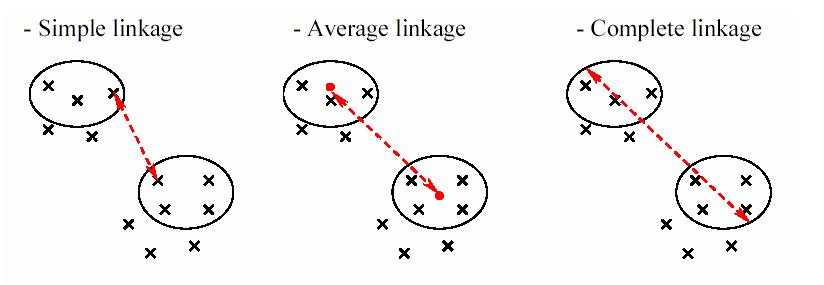
\includegraphics[width = 100mm]{linkages.jpg}
	\caption{Differenze fra i vari tipi di funzioni distanza}
	\label{linkages}
\end{figure}

\subsection{Graph Clustering}
Un grafo è una coppia ordinata $ G = (V, E)$ di insiemi, con $V$ insieme dei nodi ed $E$ insieme degli archi, tali che gli elementi di $E$ siano coppie di elementi da $V$ da $ E \subseteq V\times V$ segue in particolare che  $|E|\le |V|^2$.
\\\\
I grafi sono oggetti discreti che permettono di schematizzare una grande varietà di situazioni e di processi e spesso di consentirne delle analisi in termini quantitativi e algoritmici.
\\\\
Nello studio di reti complesse, è possibile trovare gruppi di nodi fortemente connessi, che possono essere raggruppati in comunità (potenzialmente sovrapposte). Questa disomogeneità di connessioni suggerisce che esiste una certa divisione naturale all’interno della rete. Nel caso particolare di strutture non sovrapposte, la ricerca di comunità implica la divisione della rete in gruppi di nodi con fortemente connessi internamente e connessioni sparse fra i gruppi.
Una definizione più generale è basata sul principio che coppie di nodi sono più probabilmente connessi se fanno parte della stessa comunità, e meno probabilmente connessi se non condividono la stessa comunità.
\\\\
Le comunità sono molto comuni all’interno delle reti. Le reti sociali includono gruppi di comunità che condividono la posizione, gli interessi, l’occupazione ecc. Essere in grado di individuare queste sotto-strutture all’interno di una rete può fornire indizi  su come come funziona la rete in considerazione o la topologia che influenza i nodi. Questi indizi possono essere utili per implementare algoritmi sui grafi. Molti metodi di community detection sono stati sviluppati con diversi livelli di successo.

\subsubsection{Minimum-cut method}
In questo metodo, la rete è divisa in un numero predeterminato di parti, generalmente della stessa grandezza, scelte in modo che il numero degli archi tra i gruppi è minimizzato. Questo metodo funziona bene in molte applicazioni per le quali è stato ideato, ma non è la scelta migliore per scovare comunità in reti generali, dato che troverà comunità indistintamente dal fatto che queste ci siano o meno e troverà solo un numero fissato di comunità.

\subsubsection{Hierachical-clustering}
Un altro metodo per scovare sotto-strutture conesse nelle reti viene effettuato tramite algoritmi di clustering gerarchico. Con questo approccio si definisce una misura di similarità fra coppie di nodi. Misure comunemente usate sono la coseno similarità, l’indice di Jaccard e la distanza di Hamming fra le righe della matrice di adiacenza. Poi i gruppi di nodi simili vengono raggruppati in comunità.

\subsubsection{Girvan-newman algorithm}
Un altro algoritmo molto utilizzato è quello di Girvan–Newman. Questo algoritmo identifica all’interno della rete, gli archi che uniscono community diverse e li rimuove, isolandole. L’identificazione di tali archi è effettuata applicando una misura nota della teoria dei grafi: la \textbf{betweenness centrality}. Questa assegna un valore ad ogni arco, che è alto tanto più l’arco è attraversato nel cammino più breve (geodesico) che collega due qualsiasi nodi della rete.
\begin{figure}[htb]
	\centering
	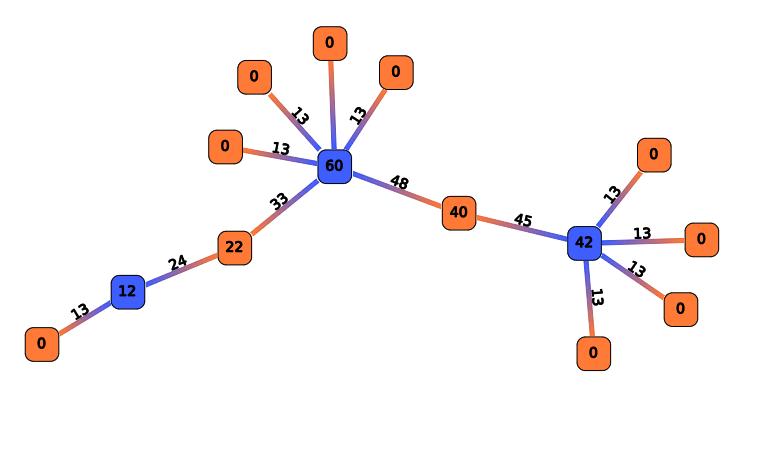
\includegraphics[width = 100mm]{betweenness.png}
	\caption{Betweenneess centrality score}
	\label{betweenness}
\end{figure}

\subsubsection{Modularity maximization}
La modularità è una misura che viene attribuita al grafo.  Questa compara la densità all’interno dei cluster con la densità fra di essi. Indica una certa divisione intrinseca e viene utilizzata per conoscere “quanto“ un grafo è separato.
\\\\
Nonostante i suoi svantaggi uno dei metodi più utilizzati per il community detection è la massimizzazione della modularità. Questo approccio scova strutture connesse tramite la ricerca della miglior divisione di una rete in modo che la modularità risulti massimizzata. 
\\\\
Dato che effettuare un confronto su tutte le possibili combinazioni è solitamente impraticabile, gli algoritmi di questa famiglia si basano su metodi di ottimizzazione approssimati quali algoritmi greedy, cioè che cercano di ottenere una soluzione ottima da un punto di vista globale attraverso la scelta della soluzione considerata migliore ad ogni passo locale. Un famoso approccio di questo tipo è il metodo Louvain, che ottimizza le community locali iterativamente, fin quando la modularità globale non può più essere migliorata. 
\\\\
L’accuratezza di questi algoritmi, comunque, è dibattuta, in quanto è stato dimostrato che molte volte fallisce nell’individuare cluster più piccola di una certa soglia, dipendente dalla grandezza della rete. 
\begin{figure}[htb]
	\centering
	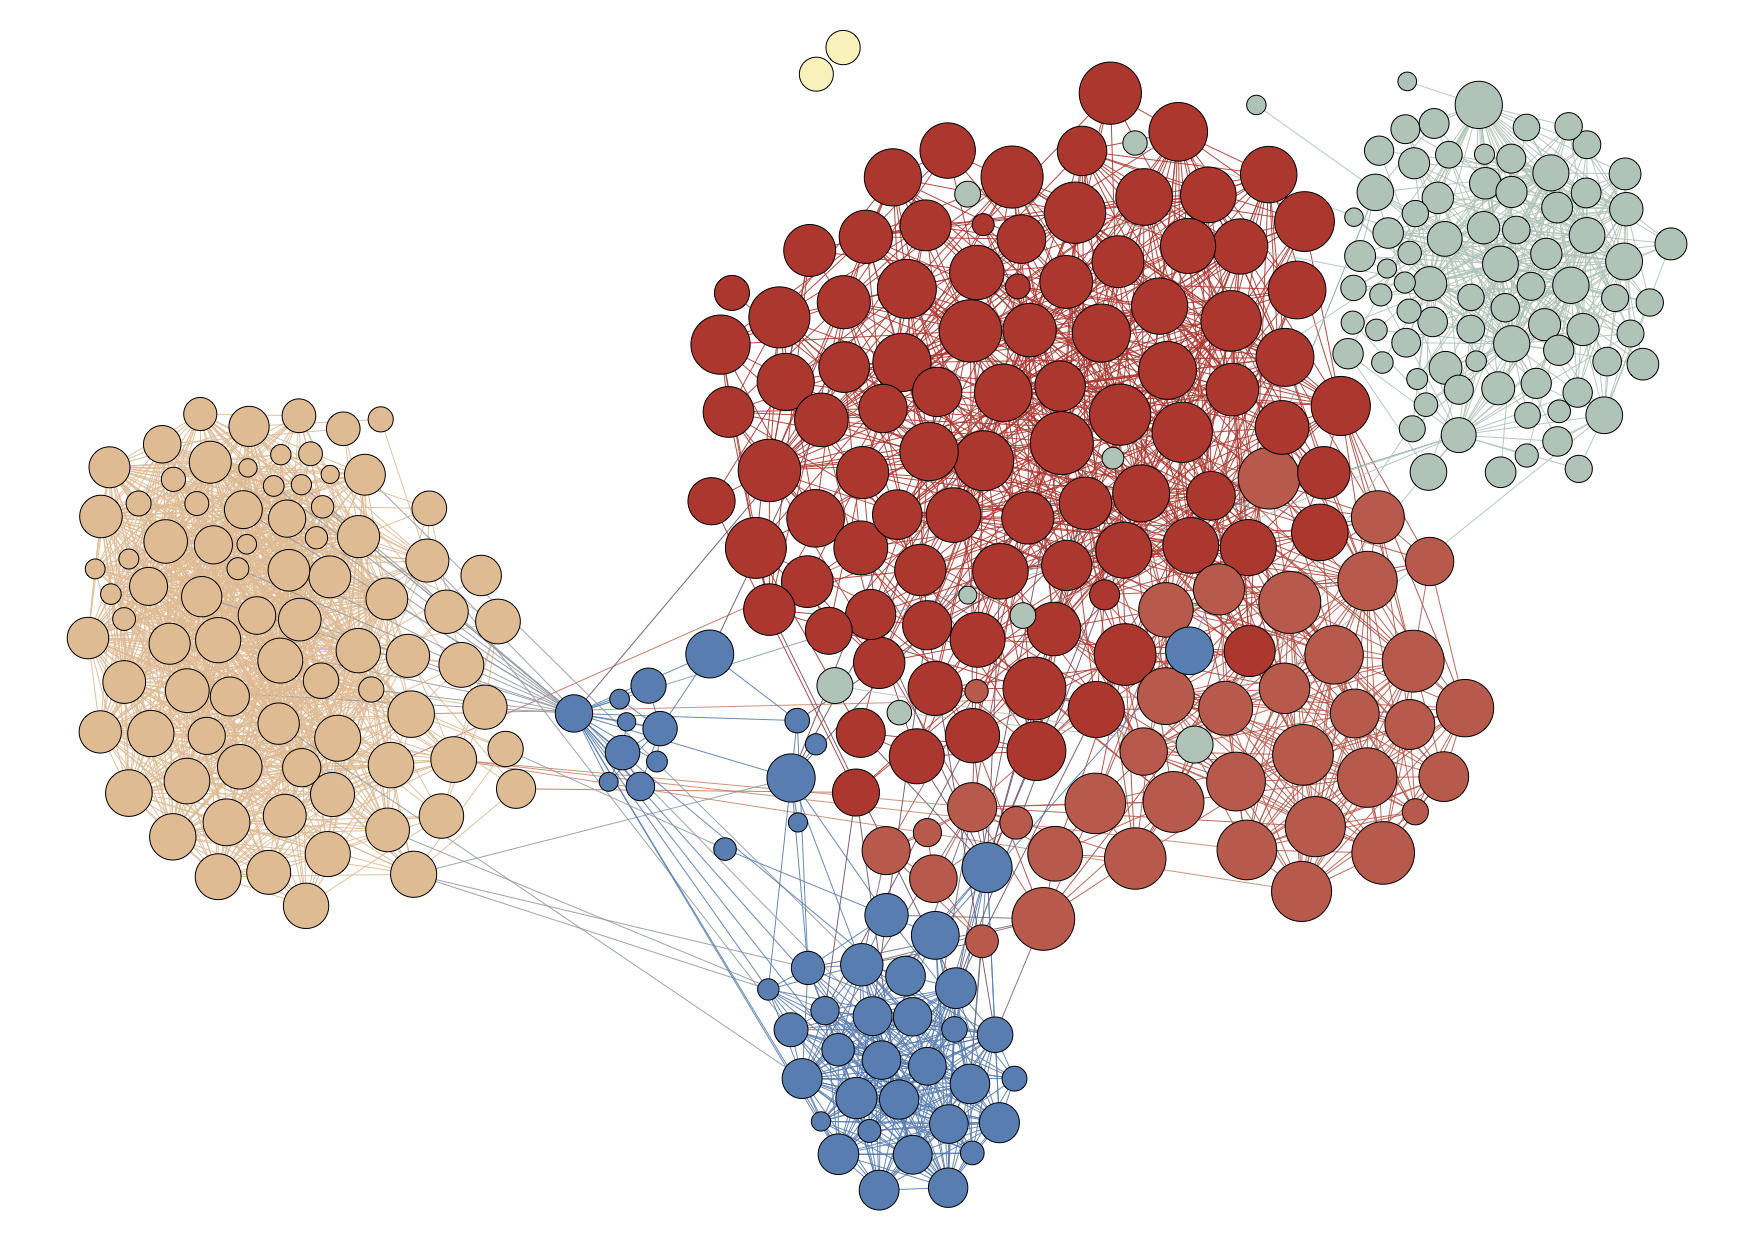
\includegraphics[width = 100mm]{modularity.png}
	\caption{Modularity score}
	\label{modularity}
\end{figure}
\subsubsection{Clique-based methods}
Le cricche (cliques) sono sottografi dove ogni nodo è collegato con ogni altro nodo nella cricca. Dato che i nodi non possono essere più connessi di così, non è sorprendente che ci siano molti metodi in community detection che si basano su questo approccio. È da notare che dato che un nodo può far parte di più di una cricca, quindi può far parte di più community contemporaneamente, questi metodi restituiscono strutture sovrapposte. 
Un approccio consiste nel trovare cricche tali che non siano sottografi di altre cricche. Un classico algoritmo per scovare tali strutture è quello di Bron-Kerbosch.



\subsection{Vector Clustering}
Gli algoritmi di clustering in uno spazio vettoriale seguono un altro approccio. Qui viene preso in considerazione la vicinanza (o la distanza) degli elementi rappresentati come punti su un iperpiano. Il feature vector associato può avere grandi dimensioni e può essere ottenuto utilizzando diverse metodologie, dipendentemente dal tipo di dato eleborato. 

\subsubsection{Hierarchical Clustering}
Anche qui il clustering gerarchico è molto utilizzato, seguendo un approccio divisivo (top-down) o agglomerativo (bottom-up), l’idea è quella di unire (o separare) elementi in base alla loro vicinanza, seguendo uno degli approcci già descritti, costruendo così una struttura chiamata dendrogramma che raggruppa gli elementi ad ogni livello. La differenza risiede nel come viene calcolata la distanza.

\subsubsection{Centroid-based clustering}
Nell’approccio basato sui centroidi, i cluster sonorappresentati da un vettore centrale, che non è neccessariamente un membro del dataset. Quando il numero dei cluster è prefissato ad un numero k, la seguente definizione formale può essere applicata: vengono definiti k centroidi e si prosegue assegnando ogni elemento al centroide più vicino, tale che il quadrato delle distanze dal cluster è minimizzato. Molti algoritmi di questa famiglia richiedono che il parametro k sia stabilito in precedenza, che è il loro più grande svantaggio. Inoltre solitamente vengono trovati cluster di grandezza simile, dato che verrà assegnato un elemento al centroide più vicino. Questi metodi partizionano lo spazio dei dati in una struttura conosciuta come diagramma di Voronoi.
\begin{figure}[htb]
	\centering
	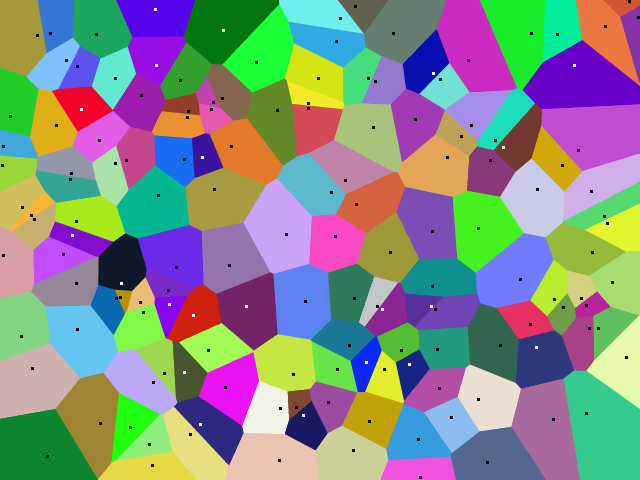
\includegraphics[width = 100mm]{voronoi.png}
	\caption{Diagramma di Voronoi}
	\label{voronoi}
\end{figure}
Nonostante questo, rimangono tra degli approcci più utilizzati ed efficaci. Da notare anche la somiglianza concettuale con l’algoritmo di classificazione KNN (k nearest neighbor).

\subsubsection{Distribution-based clustering}
Il raggruppamento avviene analizzando l'intorno di ogni punto dello spazio. In particolare, viene considerata la densità di punti in un intorno di raggio fissato. Si basano sul considerare collegati due punti che si trovano all’interno di una certa distanza limite.
I cluster sono definiti come aree con più alta densità rispetto al resto del dataset. Elementi in un area meno denso sono spesso considerati rumore, quindi come non facenti parte di nessun cluster.
\\\\
Uno degli svantaggi di questi algoritmi è che si aspettano un certo tipo di densità comune a tutti i cluster. Inoltre non eccellono nel scovare cluster presenti in molti dati del mondo reale.

\subsubsection{Document Clustering}
Agisce sempre nello spazio vettoriale, si differenzia principalmente nelle operazioni di pre-processing finalizzate ad ottenere un feature vector utilizzabile. 
Un approccio efficace consiste nel rappresentare i documenti come vettori dove ogni dimensione rappresenta la frequenza di occorrenza di una parola del vocabolario, un insieme di parole precedentemente costruito utilizzando tutte le parole del corpus. 
\begin{figure}[htb]
	\centering
	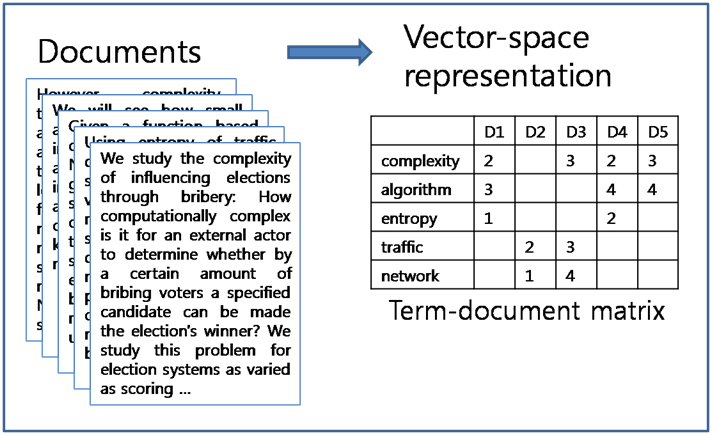
\includegraphics[width = 100mm]{tdm.png}
	\caption{Matrice termini-documenti. Ogni riga rappresenta un singolo termine ed ogni colonna rappresenta un singolo documento}
	\label{tdm}
\end{figure}

\paragraph{Term-Frequency (TF)}misura quante volte un termine appare in un documento. Dato che ogni documento ha lunghezza differente, è possibile che un termina possa apparire molte più volte nei documenti più lunghi che in quelli più corti. Quindi può essere necessario  dividere la frequenza dei termini per documenti aventi la stessa lunghezza.

\paragraph{Inverse-Document-Frequency (IDF)}un altro aspetto da considerare è a frequenza di un termine in un documento relativamente alla sua presenza globale in tutto il corpus. Tenendo in considerazione solo la frequenza di occorrenza tutti i termini sono considerati ugulamente importanti. Termini che appaiono molte volte in un documento ma meno volte in tutto il corpus potrebbero essere molto più significativi per quel specifico documento e portare molta più informazione, quindi tendono ad essere più importanti. Così come i termini che appaiono molte volte in tutti i dcoumenti del corpus sono spesso poco rilevanti e considerati inutili (stopwords).
\begin{equation}
	idf_i = \log \frac{|D|}{|\left \{ d : t_i \in d \right \}|}
\end{equation}
dove $ |D| $ è il numero di documenti nella collezione, mentre il denominatore è il numero di documenti che contengono il termine $t_i$.
Tale funzione aumenta proporzionalmente al numero di volte che il termine è contenuto nel documento, ma cresce in maniera inversamente proporzionale con la frequenza del termine nella collezione. L'idea alla base di questo comportamento è di dare più importanza ai termini che compaiono nel documento, ma che in generale sono poco frequenti.
\\\\
Altre tecniche utilizzate nel clustering sui documenti sono
\paragraph{LSI} il \textbf{Latent Semantic Indexing} è un metodo di indicizzazione e reperimento che usa una tecnica matematica chiamata decomposizione a valori singolari (SVD) per identificare pattern nelle relazioni tra i termini e i concetti contenuti in una colezione non strutturata di testo. La LSI è basata sul principio che parole che sono usate nello stesso contesto tendono ad avere significato simile. Chiamata così per la sua abilità di correlare semanticamente termini correlati che sono nascosti (latenti) in grandi collezioni testuali. La SVD può venire troncata per task di dimensionality reduction, in modo da diminuire la dimensione del vettore mantenendo comunque il significato.

\paragraph{Coseno similarità} una euristica per la misurazione della similitudine tra due vettori effettuata calcolando il coseno tra di loro. Dati due vettori di attributi numerici, $A$ e $B$, il livello di similarità tra di loro è espresso utilizzando la formula
\begin{equation}
	similarity = \cos \theta = \frac{A\cdot B}{||A||||B||}
\end{equation}
In base alla definizione del coseno, dati due vettori si otterrà sempre un valore di similitudine compreso tra $-1$ e $+1$, dove $-1$ indica una corrispondenza esatta ma opposta (ossia un vettore contiene l'opposto dei valori presenti nell'altro) e $+1$ indica due vettori uguali.
Nel caso dell'analisi dei testi, poiché le frequenze dei termini sono sempre valori positivi, si otterranno valori che vanno da 0 a $+1$, dove $+1$ indica che le parole contenute nei due testi sono le stesse (ma non necessariamente nello stesso ordine) e $0$ che non c'è nessuna parola che appare in entrambi.


\section{Data Visualization}
Un nota sulla visualizzazione dei dati, campo in crescita data la corrispondente crescita su economie basate sull’informazione e sulla crescita dei dati generati (big data) portata avanti anche da campi relativamente nuovi nel campo dell’analisi dei dati, come Business Analytics, Business Intelligence, Data Science etc.
\\\\
Tale disciplina è indirizzata a comunicare informazioni in modo chiaro e comprensibile, attraverso grafici, tabelle, diagrammi ecc. La visualizzazione può spesso aiutare ad analizzare e ragionare sui dati, rendendo dati complessi molto più accessibili ed usabili.
\begin{figure}[htb]
	\centering
	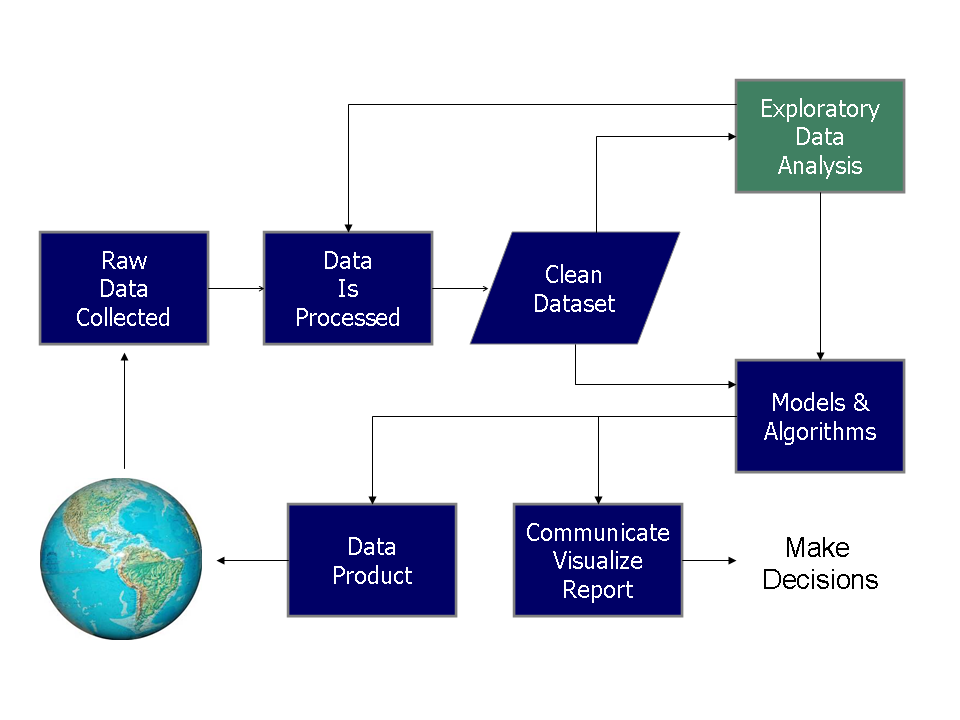
\includegraphics[width = 100mm]{datavisualization.png}
	\caption{La visualizzazione dei dati è un passo fondamentale nell'analisi dei dati.}
	\label{datavisualization}
\end{figure}



\chapter{Il Sistema Url2vec}
\label{cap:capitolo2}
% !TEX encoding = UTF-8
% !TEX TS-program = pdflatex
% !TEX root = ../Tesi.tex
% !TEX spellcheck = it-IT

%************************************************

%************************************************
%Il sistema Url2vec si propone come alternativa alle metodologie di clustering di siti web basate sul contenuto testuale delle pagine~\cite{Rajaraman11}. 
I grafi possono essere utilizzati per modellare innumerevoli fenomeni reali, da quelli scientifici a quelli sociali. Questi rappresentano le entità non come singole unità descritte appieno dalle loro caratteristiche, ma piuttosto dai collegamenti che intercorrono tra di esse. Queste ''relazioni'' codificano la maggior parte delle informazioni latenti in un grafo, caratterizzandolo in maniera univoca.

In questa tesi si approfondiscono tecniche e metodologie per le estrazione di queste informazioni dal grafo del Web, più precisamente di un sito Web, indirizzate alla divisione delle pagine in cluster omogenei. Le pagine Web tuttavia non sono divisibili in classi ben definite, non ci sono informazioni esplicite che rappresentano univocamente i professori, gli studenti o i corsi. Data questa assenza, non è possibile generare un modello accurato di classificazione. Si è rivelato necessario risolvere il problema con un latro approccio.

A dispetto della diversità delle pagine Web nella rete, quelle che risiedono all'interno di una particolare organizzazione, spesso, condividono una certa struttura. Questa può essere appresa attraverso l'analisi del peso, della densità o della direzione degli hyperlink presenti nelle pagine Web, ovvero gli archi del grafo costruito su di esse. Ad esempio, il sito Web di un dipartimento di informatica conterrà pagine riguardanti i docenti, gli studenti, i corsi, la ricerca che saranno accessibili attraverso determinati \textit{percorsi} del grafo. L'analisi dei grafi comporta anche degli svantaggi, gli algoritmi della teoria dei grafi sono NP-completi \cite{Garey}, e questo non può essere trascurato considerando le dimensioni del Web. Nella metodologia presentata viene proposta l'alternativa di apprendere rappresentazioni vettoriali dei vertici all'interno del grafo, utilizzandole insieme alle informazioni estratte dal contenuto di una pagina Web, così da processare vettori linearmente indipendenti. Queste rappresentazioni vettoriali sono apprese attraverso la generazione di percorsi attraverso gli archi del grafo, creando delle sequenze di vertici che saranno trattate come frasi, dove le parole sono pagine Web. 


\subsection{NLP nel Web: URL Embedding}
In questo modo è possibile sfruttare i recenti sviluppi nel campo del Word Embedding. Questi algoritmi riescono a considerare sempre più fattori e restituire vettori sempre più accurati. Vengono incluse informazioni riguardanti il contesto di una parola, ovvero gli altri termini contenuti nella frase in cui compare la parola analizzata. Nel Web questo implica considerare le pagine ''più vicine'', ovvero le pagine che puntano o sono puntate direttamente dalla pagina in esame, privilegiando quelle che hanno più collegamenti con questa. Questa informazione riesce ad estrarre le informazioni latenti nella struttura del sito, ed a raggruppare le pagine similmente ad un algoritmo di partizionamento di un grafo. Queste informazioni hanno rivelato proprietà peculiari quando applicate su grandi testi. Il caso più noto e controverso è quello delle analogie. 

È stato osservato che correlazioni nascoste possono trovarsi nella differenza tra coppie di vettori~\cite{Mikolov13}, come nel caso di parole simili ma con leggere differenze come il genere o il numero, infatti esse appaiono in frasi tendenzialmente simili, ma con delle piccole differenze. In questo caso l'informazione può essere interpretata come il genere o il numero.
\\\\
Informazioni simili possono essere trovate anche nel campo del Web. È ormai consolidata la questione dell'autorità di alcune pagine~\cite{Kleinberg99} e di come queste abbiano un maggior numero di link in entrata. Alcune pagine tuttavia saranno accessibili prevalentemente attraverso alcuni percorsi e si troveranno quindi in un contesto con elementi simili. Il problema resta dare un senso a queste correlazioni ed un significato utilizzabile. Nello sviluppo di Url2vec, tuttavia, sono emerse corrispondenze abbastanza naturali, come le pagine dei professori con i relativi corsi insegnati o i laboratori di afferenza. 

Queste relazioni sono dovute al fatto che il grafo di un sito Web è fortemente connesso, ma la maggior parte delle volte in cui appare un determinato corso di studio appare anche il relativo docente e viceversa. 

\subsubsection{Differenza tra parole ed URL}
La sola analisi delle sequenze comunque può risultare limitata. Le pagine Web non sono parole, ad esse è associata un ulteriore informazione, ovvero il contenuto testuale. Questa proprietà si è rivelata molto utile, infatti combinando le informazioni ricavate dall'esame di tutti e due gli aspetti, il grado di accuratezza del processo di clustering è salito in modo significativo. Il contenuto di una pagina infatti fornisce informazioni fondamentali su di essa, ma queste possono variare significativamente anche tra pagine considerate dello stesso tipo, presentando ad esempio una diversa distribuzione dei termini. Analizzando la struttura connessa delle pagine Web, si è cercato costruire delle rappresentazioni più significative.
%https://www.ideals.illinois.edu/bitstream/handle/2142/45402/Timothy_Weninger.pdf?sequence=1}
%The parallel path framework for entity discovery on the Web
Saper sfruttare tale struttura può agevolare notevolmente i task di Web Mining. Esso infatti estrae conoscenza strutturata e facilmente processabile.

%A partire da questo punto stai per descrivere il COME hai realizzato il tuo sistema, peccato che manca il COSA, ossia cosa fa il tuo sistema, cosa hai fatto di interessante, in che modo il tuo sistema è capace di superare delle open challenges, ect.
Nelle sottosezioni che seguono si descrive il sistema realizzato, oltre che le tecniche e gli algoritmi utilizzati per la realizzazione degli obiettivi preposti.\\
Sono state realizzate tre macro componenti.
\begin{itemize}
\item \textit{Crawling delle pagine Web}. Questo è regolato da alcuni parametri che rendono il processo flessibile e altamente modificabile.
\item \textit{Costruzione del Dataset}, ovvero la strutturazione delle informazioni ottenute nel processo precedente, secondo alcuni criteri necessari per le successive elaborazioni.
\item \textit{Clustering delle pagine Web} attraverso la combinazione dell'analisi del contenuto testuale e delle relazioni tra le pagine.
\end{itemize}

\section{Web Crawling per l'estrazione dei dati}
\label{crawling}
Le proprietà che caratterizzano le pagine Web rendono complicato il processo di estrazione di informazioni, soprattutto nel caso in cui i contenuti vengono generati dinamicamente.

\begin{figure}[htb]
	\centering
	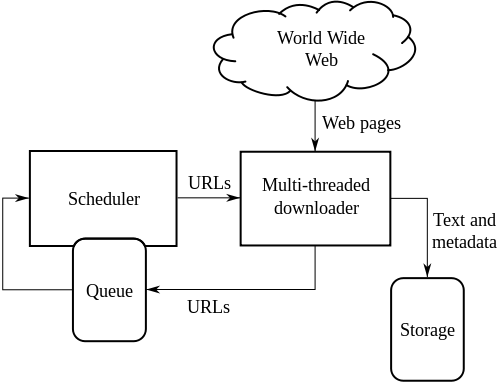
\includegraphics[width = 100mm]{crawlerarch.png}
	\caption{Architettura di un web crawler}
	\label{crawlerarch}
\end{figure}

Un Web crawler, chiamato anche web spider o web robot, è un componente software. I suoi obiettivi principali sono:
\begin{itemize}
\item raccogliere il più velocemente ed efficientemente possibile pagine utili, insieme alla struttura ad hyperlink che le collega;
\item copiare tutte le pagine che visita per elaborazioni future, per poi indicizzarle cosi che gli utenti possano trovarle più velocemente;
\item validare gli hyperlink e il codice HTML;
\item eseguire il Web Scraping delle pagine Web.
\end{itemize}

Esso esplora una pagina alla volta, analizandone la struttura e gli hyperlink contenuti. Questi sono immagazzinati nella ''frontiera'' che inizialmente vuota, conserva tutte le pagine ancora da esplorare. L'ordine di esplorazione e le politiche di filtraggio degli hyperlink possono variare in base al risultato desiderato. 

\begin{algorithm}[H]
\caption{Crawling BFS}
\begin{algorithmic}

	\State $url\gets homepage$;	\Comment{Pagina da cui iniziare}
	\State $queue\gets empty$ \Comment{Coda per la BFS}
	\State $analyzedVertex.add(url)$;	\Comment{Insieme di url già visitati}
	\State $maxDepth url$;	\Comment{Massima profondità di esplorazione}
 	
 	\vspace*{+0.5cm}
 	
	\State \textbf{Begin}
	\While{$queue \neq empty$} 
		\State $urlToAnalyze\gets queue.dequeue()$
		
		\If{$urlToAnalyze.depth \leq maxDepth$}
			\State $outlinks \gets urlToAnalyze.getOutlinks()$
		\Else
			\State $urlToAnalyze$
		\EndIf
		\If{$outlinks \neq null$}
			\State $outlinks \gets urlToAnalyze.getOutlinks()$
			\State $analyzedVertex.add(outlinks)$
			\State $serialize(urlToAnalyze)$
			\For{\textbf{each} link in outlinks}
				\State $serialize(link)$
				\State $queue.enqueue(link, urlToAnalyze + 1)$
			\EndFor
		\EndIf
		
	\EndWhile
	\State \textbf{End}
\end{algorithmic}
\end{algorithm}

\subsection{Proprietà del web crawler}
Nel processo di Crawling, data la natura non strutturata del Web, è necessaria l'applicazione di numerose tecniche e metodologie per un corretto funzionamento.

\subsubsection{Normalizzazione degli URL}
Il termine di normalizzazione, chiamato anche canonicalizzazione di URL, si riferisce al processo di modifica e standardizzazione di un URL in una maniera consistente, ad esempio alcuni siti Web mettono a disposizione gli stessi file o i medesimi contenuti attraverso URL differenti. 
\\\\
\texttt{http://domain.com/products/page.php?product=smartphone}
\\
\texttt{http://domain.com/products/smartphone.php}
\\\\
\texttt{http://www.domain.edu/courses}
\\
\texttt{http://www.domain.edu/courses/index.html}
\\\\
Le due coppie di URL nell’esempio puntano agli stessi contenuti. Altri casi sono URL che differscono solo per il protocollo (''\texttt{http://}'' o ''\texttt{https://}'') o l'omissione della stringa ''\texttt{www}''. Effettuando la normalizzazione, si sceglie un URL come formato di riferimento per accedere ad un determinato contenuto. Ci sono diversi tipi di normalizzazione che possono essere usati, come la conversione in minuscolo, rimuovere i ''.'' e ''..'' portando gli URL relativi ad URL assoluti, aggiungere slash finali al componente di percorso non vuoto.
\\\\
Una soluzione consiste nella creazione di un dizionario che ha come chiavi gli hashcode del contenuto testuale delle pagine e come valori una lista di tutti i diversi URL che hanno quel contenuto. In questo modo si riduce il problema ad una sola operazione così da annullare le relazioni e i vari di pattern da scovare nall'analisi degli URL per capire se sono la stessa pagina o meno. 

\subsubsection{Ricerca all'interno dello stesso dominio}
Per estrarre informazione e per il successivo processo di clustering delle pagine web, è necessario che le pagine estratte si riferiscano allo stesso dominio, o in altri termini, che appartengano allo stesso sito web.
\\
Questo viene effettuato per sfruttare la struttura gerarchica del dito web rivolto principalmente riuscire a  raccogliere le informazioni nascoste nel grafo e sopratutto negli hyperlink.

\subsubsection{Dimensione della ricerca}
Anche limitando la ricerca ad un solo dominio, la dimensione delle pagine da esplorare, e quindi la grandezza della frontiera, può aumentare considerevolmente o addirittura portare il processo di crawling a divergere.

\begin{figure}[htb]
	\centering
	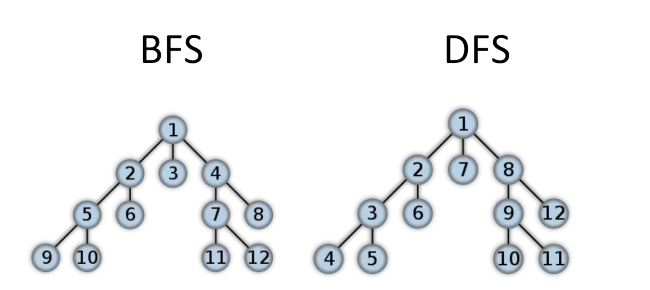
\includegraphics[width = 100mm]{breadthdepth.png}
	\caption{Differenze tra ricerca in ampiezza e ricerca in profondità}
	\label{breadthsearch}
\end{figure}

È stata utilizzata una ricerca in ampiezza con un limite variabile di profondità. Ponendo un limite all'esplorazione del grafo delle pagine si garantisce la la terminazione del processo di crawling e utilizzando una ricerca in ampiezza si dà priorità alle pagine vicine al nodo radice (comunemente l'homepage). Questa scelta è stata dettata anche dal cercare di evitare le cosiddette ''spider traps''. Queste sono dei meccanismi utilizzati, intenzionalmente o involontariamente, dai server oggetto di crawling, che possono portare ad una generazione dinamica e potenzialmente infinita in URL univoci, e quindi considerati come pagine diverse. Questo può essere evitato non aggiungendo alla frontiera URL che contengono il carattere ''?'', ma questo non è sempre efficace.
\\\\
Inoltre è stato osservato che nei siti web entity-oriented, le informazioni ricercate si trovano quasi sempre nei primi livelli di gerarchia \cite{He13}.

\subsubsection{Restrizione dell'esplorazione}
La restrizione può essere effettuata sulle pagine da esplorare o dalla frequenza di richieste che è possibile effettuare.
\\\\
Il robots exclusion protocol è uno standard che consiste in un file (robots.txt), posto alla radice della gerarchia di un sito Web. In pratica, il file indica le regole utilizzate dai crawler per applicare restrizioni di analisi sulle pagine di un sito web. 
\\\\
Molte volte i crawler non sono ben accetti, in quanto possono rallentare pesantemente la navigazione. Se server effettua dei controlli sulle richieste ricevute e queste hanno una frequenza troppo elevata o seguono uno schema riconducibile ad una macchina queste possono essere ignorate. Può capitare che richieste continue e non curanti delle restrizioni imposte portino a bandire l'indirizzo IP del servizio trasgressore.\\
Per evitare tali conseguenze è opportuno seguire una certa etica nell'operazione di crawling.

\subsection{Estrazione delle liste}
\label{liste}
Riuscire a strutturare dati non strutturati può rivelarsi ostico. Molti tentativi, più o meno efficaci, sono stati effettuati a tale proposito.
\\
In questa tesi uno degli obiettivi è stato quello di prendere in considerazione i collegamenti all'interno delle pagine web, seguendo i percorsi generati dalla concatenazione di più hyperlink. Questa scelta è stata effettuata sulla base dei recenti progressi nel campo del natural language processing (NLP)~\cite{Turian10}. Esplorando la struttura del grafo del web, data la forte connessione che esiste fra i suoi nodi, estrarre informazione può rivelarsi un operazione tutt'altro che banale. 
\\\\
È stato utilizzato il concetto di \textbf{lista}. 
Per permettere una migliore visualizzazione dell'informazione descritta, quasi tutte le pagine Web vengono formattate utilizzando regole CSS. Di conseguenza, per poter effettuare correttamente questo task, bisogna prima elaborare la pagina Web con tutte le informazioni grafiche sui nodi HTML e solo successivamente si può procedere alla loro estrazione. Grazie alle informazioni ricavate dall’HTML della pagina Web e dalla posizione e dimensione dei singoli nodi, è possibile stabilire una struttura gerarchica ad albero dei nodi che la compongono. Questa struttura gerarchica ad albero permette di scoprire i record, ovvero dati strutturati (ad esempio provenienti da database) che sono allineati orizzontalmente, verticalmente e anche strutturalmente (elementi HTML ul, li, . . . ); permette quindi di individuare dei gruppi di record, ovvero delle liste di record.
\\
L’individuazione delle liste di raggiungere pagine che contengono elementi simili a quelli contenuti nella pagina che si sta visualizzando. 
In questo modo le pagine dovrebbero essere accessibili solo attraverso percorsi predeterminati e non in maniera fortemente connessa. I nodi e gli archi risultanti risultano così un sottoinsieme di quelli originali.

\section{Costruzione del Dataset}
I dati estratti nel processo vanno organizzati e ampliati in modo da garantire l'accesso e l'elaborazione in maniera agevole.
\\
Il processo di crawling restituisce il grafo delle pagine web e il contenuto testuale di ogni pagina esplorata, a queste va aggiunta la generazione delle sequenze attraverso la teoria dei \textit{Random Walk}, come spiegato in \ref{rwsection}. Inoltre per un minor spreco di risorse si è optato per la conversione degli URL in codici, ovvero una associazione univoca fra un URL ed un codice (e.g. un numero) molto più corto, così da risparmiare tempo di elaborazione e spazio di archiviazione.

\subsection{Random Walk}
\label{rwsection}
Per la generazione delle sequenze è stato utilizzata la teoria dei \textit{Random Walk}. In matematica, un Random Walk è la formalizzazione dell'idea di prendere passi successivi in direzioni casuali. Matematicamente parlando, è il processo stocastico più semplice, il processo markoviano. Qui sono utilizzati per ricavare percorsi pseudo casuali da attraversamento del grafo del web per ottenere sequenze di URL collegati semanticamente.
\\\\
In una passeggiata aleatoria monodimensionale si studia il moto di una particella puntiforme vincolata a muoversi lungo una retta nelle due direzioni consentite. Ad ogni movimento essa si sposta (a caso) di un passo a destra (con una probabilità fissata $\ p$) o a sinistra con una probabilità $\ 1-p$, ed ogni passo è di lunghezza uguale e indipendente dagli altri.
\begin{figure}[htb]
	\centering
	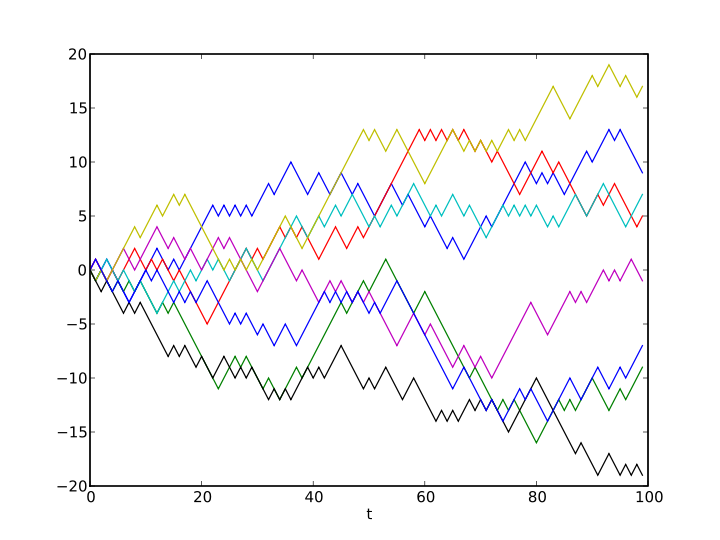
\includegraphics[width = 100mm]{randomwalkonedim.png}
	\caption{Rappresentazione visuale di 8 random walk monodimensionali. }
	\label{englishchinese}
\end{figure}
\\\\
In una passeggiata aleatoria bidimensionale si studia il moto di una particella vincolata a muoversi sul piano spostandosi casualmente ad ogni passo a destra o a sinistra con probabilità $\frac{1}{2}$, verso l'alto o verso il basso con probabilità $\ p=\frac{1}{2}$. In pratica ad ogni passo può compiere un movimento lungo una delle quattro diagonali con probabilità $\frac{1}{4}$. Ci si chiede con che probabilità la particella tornerà al punto di partenza.
\begin{figure}[htb]
	\centering
	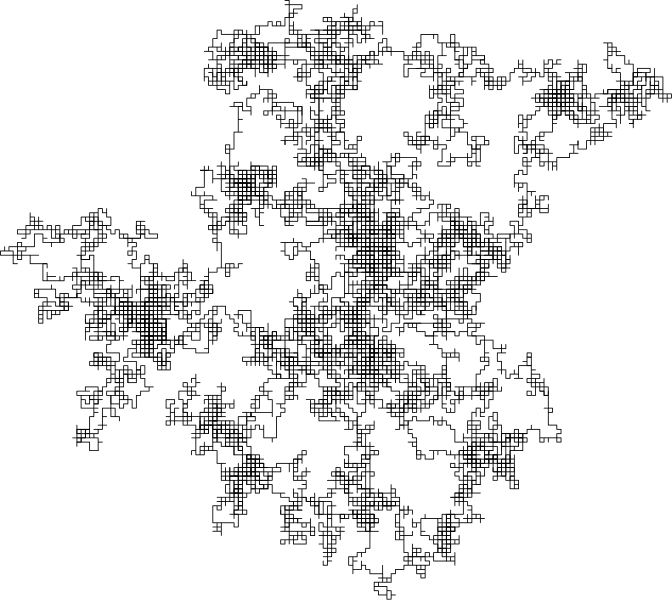
\includegraphics[width = 100mm]{randomwalktwodim.png}
	\caption{Rappresentazione visuale di un random walk di 25.000 passi su due dimensioni. }
	\label{englishchinese}
\end{figure}
\\\\
Queste passeggiate aleatorie possono trovare effettivi riscontri in natura come il traiettoria percorso da una particella in un liquido o in un gas, il tragitto di un animale affamato o anche il prezzo di un titolo fluttuante o la situazione finanziaria di un giocatore d'azzardo. Tutti questi esempi possono essere espressi come random walk, anche se in natura potrebbero non essere veramente casuali.
\\\\
Un popolare modello di random walk è quello su un reticolo regolare, dove ad ogni passo si segue un determinato percorso basandosi su una qualche distribuzione di probabilità. Nel caso più semplice si può solo “saltare” sul sito vicino. In un semplice random walk simmetrico in un reticolo localmente finito, le probabilità di saltare su ognuno dei siti vicini è la stessa.
\\\\
Per definire un random walk formalmente, prese indipendenti variabili casuali $ Z_1, Z_2, Z_3, $ \dots dove ogni variabile è o 1 o -1, con una probabilita del 50\% per ognuno dei due casi, e dato 
\begin{equation}
  S_0 = 0
\end{equation}
\begin{equation}
  S_n = \sum_{j=1}^{n} Z_j
\end{equation}
  
la serie $\left \{ S_n \right \} $ è chiamata random walk semplice in $\mathbb{Z}$.
\\\\
Si consideri un attraversatore casuale della rete (random surfer) che, partendo da un pagina web, esegue un passo alla volta in questo modo: ad ogni iterazione, dalla pagina corrente, procede verso una pagina a caso tale che esiste un link che dalla pagina corrente punta a questa.
\\\\
Procedendo da pagina a pagina, visiterò alcuni nodi, più spesso di altri; intuitivamente, saranno nodi con molti link entranti da altri nodi frequentemente visitati. Ci sono alcuni problemi. Che succede se si arriva ad una pagina che non ha link in uscita? In questo caso è necessario introdurre un’altra operazione: il teletrasporto. In questa operazione l’attraversatore casuale salta dal nodo corrente ad un qualsiasi altro nodo sulla rete.
Se $N$ è il numero totale dei nodi nel grafo, l’operazione di teletrasporto porta l’attraversatore verso ogni nodo con probabilità $\frac{1}{N}$. Potrebbe anche trasportarsi sulla posizione corrente con probabilità di $\frac{1}{N}$. Questa operazione è chiamata quando si arriva ad un non senza nodi in uscita o con una probabilità$\ d$ data, con$\ 0 < d < 1$.


\subsection{Generazione delle sequenze}
Le sequenze rappresentano un percorso che un attraversatore casuale della rete seguirebbe cliccando su un hyperlink a caso fra tutti quelli disponibili nella pagina corrente (o eventualmente nelle liste). Questi percorsi, chiamati \textbf{Random Walk} (o passeggiate aleatorie), sono stati largamente utilizzati in molti algoritmi sui grafi e sul Web~\cite{aldous14} in quanto buone approssimazioni di comportamenti casuali. Il problema di questa tecnica applicata al Web si presenta quando l'attraversatore casuale arriva ad una pagina priva di hyperlink. La soluzione più diffusa consiste nell'effettuare un ''salto'' verso una qualsiasi altra pagina quando non ci sono outlink da seguire. 
\\\\
Qui il problema non si pone, in quanto le sequenze generate hanno una lunghezza fissata prima dell'esecuzione e se la generazione dovesse bloccarsi, la sequenza risultante sarà solo più piccola. Questa scelta è dovuta dal fatto che l'informazione cercata scaturisce da percorsi reali di navigazione e non necessita una lunghezza obbligatoria da rispettare, in quanto le sequenze possono essere viste come frasi di un testo, dove le parole sono gli URL.
\\\\
Per motivi di sperimentazione sono stati implementati tre tipi diversi di Random Walk, utilizzabili modificando i parametri di esecuzione dell'algoritmo.



\begin{algorithm}[H]
\caption{Generazione delle sequenze}
\begin{algorithmic}

	\State $numRandomWalks$;	\Comment{Numero di Random Walk da generare}
	\State $lengthRandomWalks$ \Comment{Lunghezza dei Random Walk}
 	
 	\vspace*{+0.5cm}
 	
	\State \textbf{Begin}
	\State $node \gets \Call{randomnode}{}$
	\For{$i \gets 0 \to numRandomWalks$} 
		\State $sequence.add(node)$
		
		\While{$sequence.length \leq lengthRandomWalks$}
			\If{$node.hasOutlinks()$}
				\State $node \gets node.getOutlinks(RandomIndex)$
				\State $sequence.add(node)$
			\Else
				\State $break$
			\EndIf
		\EndWhile
		\State $serialize(sequence)$
		
	\EndFor
	\State \textbf{End}
\end{algorithmic}
\end{algorithm}


\subsubsection{Random Walk standard}
Questo è il caso standard, ovvero si parte da un nodo casuale del grafo e si segue ogni volta un arco a caso fra quelli disponibili, fino al raggiungimento della lunghezza prefissata o all'impossibilità di proseguire.
\\
Da notare che questo processo e il precedente non sono completamente separati, in quanto la scelta di un nodo casuale e la consecutiva traiettoria, possono portare all'esplorazione di pagine non precedentemente visitate. È quindi necessario mantenere aggiornato il grafo immagazzinato.
\begin{figure}[htb]
	\centering
	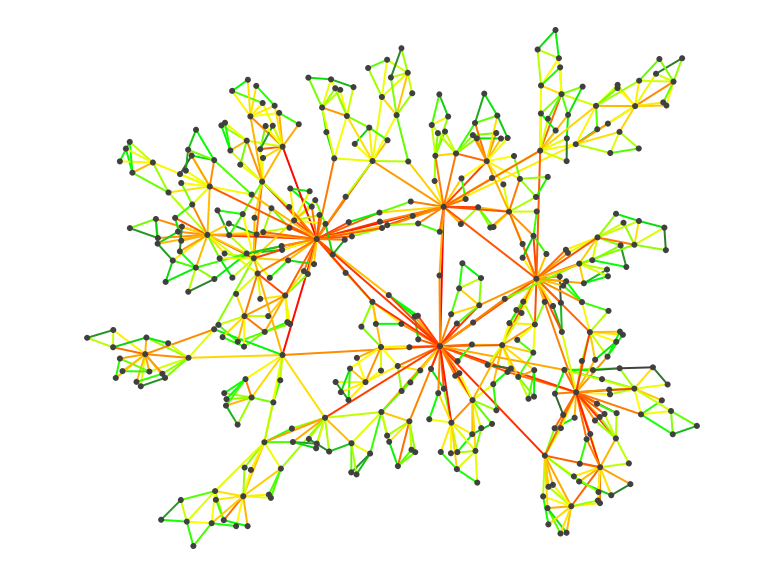
\includegraphics[width = 100mm]{randomWalkongraph.png}
	\caption{Random walk sul grafo. }
	\label{englishchinese}
\end{figure}
\subsubsection{Random Walk con partenza fissa}
Qui l'unica differenza consiste nel punto di partenza del cammino. Infatti si può partire in un nodo prefissato del grafo (generalemnte l'homepage di un sto web), in modo da esplorare più percorsi possibili avente quel nodo come origine.

\subsubsection{Random Walk attraverso le Liste}
Qui invece si può seguire uno dei due approcci precedenti, ma con il vincolo delle liste, quindi limitando la camminata ad un sottoinsieme di quella precedente.

\subsection{Esempio di Dataset}
Di seguito sono elencati file generati nel processo di crawling e di generazione delle sequenze. Gli esempi riportati di seguito sono stati ottenuti analizzando il sito del dipartimento di informatica di Urbana, IL: \texttt{www.cs.illinois.edu}

\subsubsection{urlsMap.txt}
Contiene la associazioni fra gli URL e il relativo codice identificativo. Questo è dovuto dalle ragioni spiegate in precedenza, ovvero ridurre i tempi di elaborazione e spazio di archiviazione. 
\\\\
\texttt{
http://cs.illinois.edu,3\\
http://cs.illinois.edu/prospective-students,4\\
http://cs.illinois.edu/current-students,5\\
http://cs.illinois.edu/courses,6\\
http://cs.illinois.edu/alumni,7\\
http://cs.illinois.edu/research,8\\
http://cs.illinois.edu/news,9\\
http://cs.illinois.edu/partners,10\\
http://cs.illinois.edu/about-us,11\\
. . .\\
}
\subsubsection{vertex.txt}
Contiene il contenuto testuale di ogni pagina esplorata. Ogni riga è quindi formata da il codice identificativo di un URL e il relativo contenuto.
\\\\
\texttt{
1	department of computer science at illinois engineering at ...\\
2	prospective students department of computer science at ...\\
3	current students department of computer science at ...\\
4	courses department of computer science at illinois ...\\
5	alumni department of computer science at illinois ...\\
6	research department of computer science at illinois    ...\\
7	news department of computer science illinois engineering ...\\
8	partners department of computer science at illinois ...\\
9	about us department of computer science at illinois ...\\
. . .\\
}
\subsubsection{edges.txt}
Questo è il file principale per la generazione delle sequenze, qui sono immagazzinate tutte le relazioni fra le pagine, ovvero gli archi che le collegano. 
\\\\
\texttt{
1	1\\
1	2\\
1	3\\
1	4\\
1	5\\
1	6\\
1	7\\
1	8\\
1	9\\
. . .\\
}
\subsubsection{sequencesIDs.txt}
Contiene le sequenze generate. I codici relativi alle pagine web sono separati da '' -1 '' e la linea finisce con un '' -2 ''. Da notare che sono riportate le sequenze che partono da un nodo casuale del grafo.
\\\\
\texttt{
137 -1 2 -1 27 -1 8 -1 52 -1 53 -1 8 -1 8 -1 10 -1 13 -1 -2\\
506 -1 5 -1 14 -1 11 -1 6 -1 2 -1 27 -1 114 -1 111 -1 11 -1 -2\\
424 -1 4 -1 12 -1 6 -1 8 -1 53 -1 4 -1 7 -1 12 -1 8 -1 -2\\
616 -1 5 -1 6 -1 8 -1 8 -1 9 -1 1 -1 21 -1 6 -1 3 -1 -2\\
51 -1 7 -1 7 -1 38 -1 38 -1 25 -1 103 -1 27 -1 113 -1 12 -1 -2\\
429 -1 10 -1 3 -1 6 -1 4 -1 11 -1 8 -1 9 -1 9 -1 3 -1 -2\\
783 -1 421 -1 5 -1 9 -1 7 -1 5 -1 2 -1 8 -1 2 -1 24 -1 -2\\
506 -1 5 -1 8 -1 52 -1 53 -1 25 -1 40 -1 13 -1 11 -1 13 -1 -2\\
638 -1 63 -1 153 -1 62 -1 63 -1 152 -1 63 -1 155 -1 13 -1 7 -1 -2\\
. . .\\
}
\subsubsection{sequencesIDsFromHomepage.txt}
Contiene le sequenze generate che partono da uno stesso nodo. La generazione di questo file avviene esplicitando il nodo di origine di ogni sequenza nella fase di generazione.
\\\\
\texttt{
1 -1 8 -1 2 -1 14 -1 2 -1 2 -1 10 -1 14 -1 66 -1 3 -1 -2\\
1 -1 18 -1 39 -1 8 -1 8 -1 24 -1 1 -1 4 -1 7 -1 25 -1 -2\\
1 -1 23 -1 -2\\
1 -1 16 -1 10 -1 3 -1 29 -1 29 -1 4 -1 25 -1 97 -1 108 -1 -2\\
1 -1 20 -1 20 -1 1 -1 11 -1 3 -1 2 -1 9 -1 10 -1 13 -1 -2\\
1 -1 25 -1 48 -1 48 -1 44 -1 42 -1 4 -1 7 -1 38 -1 38 -1 -2\\
1 -1 25 -1 115 -1 4 -1 11 -1 11 -1 1 -1 2 -1 26 -1 13 -1 -2\\
1 -1 24 -1 4 -1 9 -1 60 -1 56 -1 6 -1 25 -1 113 -1 116 -1 -2\\
1 -1 21 -1 25 -1 135 -1 32 -1 13 -1 4 -1 25 -1 149 -1 59 -1 -2\\
. . .\\
}


\section{Web page Clustering}
%In questa sezione si parlerà della soluzione proposta come alternativa alle normali tecniche di clustering delle pagine Web basate esclusivamente sul contenuto testuale. Infatti il fulcro del sistema è basato su metodologie nate nel campo del \textbf{Natural Language Processing} ma applicate nel contesto Web, in modo da aggiungere
Il clustering delle pagine Web all'interno di uno stesso dominio può venire effettuato sfruttando la struttura connessa del sito o trattando le singole pagine Web come documenti. Nel primo caso si tratta principalmente di utilizzare algoritmi e tecniche derivanti dalla teoria dei grafi per partizionare il grafo, in modo da isolare i cluster di pagine ''simili''. Nel secondo caso invece viene analizzato unicamente il contenuto testuale visivo della pagina, si costruisce una collezione di documenti, un vocabolario dei termini e si considera ogni pagina indipendentemente dalle altre.

Gli hyperlink tra le pagine di uno stesso sito sono tipicamente utilizzati per organizzare i contenuti e puntano a contenuti inerenti ma non per forza simili. Mentre il contenuto testuale, data l'ambiguità del linguaggio naturale, può fornire indizi sbagliati e considerare diverse pagine correlate solo per una differente distribuzione dei termini.

In questa tesi si è scelto un approccio diverso, la rappresentazione di ogni pagina infatti viene creata unendo le informazioni sulla struttura della pagina all'interno del grafo con le informazioni sul contenuto testuale. È importante notare che non si applicano tecniche di partizionamento del grafo, le relazioni tra le pagine vengono apprese mediante i Random Walk generati nella fase precedente e codificate in uno spazio vettoriale. Questo comporta numerosi vantaggi computazionali. Inoltre in questo modo è possibile unire queste rappresentazioni con quelle basate sulla frequenza dei termini. In particolare le sequenze generate attraverso la teoria dei Random Walk, vengono trattate come frasi ed analizzate con tecniche di Word Embedding derivanti dal campo del Natural Language Processing. La rappresentazione vettoriale di ogni pagina non è umanamente comprensibile come la rappresentazione termini-documenti, ma è conveniente da elaborare. Queste sono state le premesse alla base del lavoro svolto, ovvero unire tecniche consolidate in aree specifiche e trasferire la conoscenza in altri domini applicativi.

L'algoritmo implementato prende in input l'insieme delle pagine, con il relativo contenuto, e le sequenze di Random Walk generate, restituendo rappresentazioni vettoriali per ogni pagina. La fase di apprendimento può comunque essere opportunamente personalizzata considerando maggiormente uno dei due aspetti o gli algoritmi utilizzati per ognuno. Questo è dovuto all'eterogeneità del Web. Infatti è stato notato che non tutti i siti tendono a formare cluster sferici, o ancora che l'organizzazione interna di un sito non sia sufficientemente informativa.

\chapter{Related works}
\label{cap:capitolo3}
% !TEX encoding = UTF-8
% !TEX TS-program = pdflatex
% !TEX root = ../Tesi.tex
% !TEX spellcheck = it-IT

%************************************************

%************************************************

Il clustering di pagine Web non è un nuovo ambito di ricerca. Nei diversi anni si sono susseguite in letteratura una serie di tecniche e metodologie per il raggruppamento ed il reperimento di pagine Web~\cite{Banos03,Cooley03,Mobasher01,chiang15,Crescenzi05}. 

Tuttavia gli sforzi si sono concentrati prevalentemente su pagine provenienti da diversi siti Web. Relativamente poco è stato il lavoro svolto sul clustering di un specifico sito di una determinata organizzazione. L'analisi degli hyperlink, infatti, ha significati diversi in relazione al domino di destinazione. Se la pagina puntata si trova nello stesso dominio, il collegamento avrà funzione di organizzazione dei contenuti, mentre se il collegamento punta ad una pagina esterna, questo sarà indirizzato alla conferma del contenuto mostrato e presenterà molto probabilmente argomenti simili~\cite{}. 

%Scoprire correlazioni nelle pagine Web può essere effettuato attraverso l'analisi del contenuto testuale e/o HTML delle pagine web. Compito degli algoritmi di clustering che analizzano il solo contenuto testuale %delle pagine web è quello di analizzare la distribuzione dei termini delle singole pagine web e raggruppare le stesse in funzione dei topic descritti. I cluster così ottenuti sono composti da pagine non necessariamente collegate tra loro, ma trattanti simili argomenti. 

%Gli algoritmi di clustering che analizzano la struttura HTML delle pagine web possono sfruttare due importanti proprietà: \textit{i) } proprietà visuali, ossia come una pagina è renderizzata da un web browser; \textit{ii) } proprietà strutturali, ossia la struttura dei tag HTML di cui una pagina web si compone. Compito degli algoritmi di clustering che ricadono in questa tipologia è  scoprire pattern di tag HTML e raggruppare le pagine web in funzione dei pattern estratti.

%Gli svantaggi di queste metodologie derivano dall'eterogeneità del Web e dalle assunzioni di partenza. Infatti la struttura a grafo fortemente connessa di un sito web può non bastare a codificare tutte le informazioni necessarie. Inoltre le assunzioni di indipendenza dei documenti nella collezione e dei termini nel documento non sono sempre verificate, soprattutto nel contesto del Web. 

Gli algoritmi di clustering di pagine web possono essere classificati in tre grandi categorie in base alle informazioni che questi utilizzano per raggruppare le pagine web:

%Le tecniche diffuse in letteratura possono dunque essere raggruppate in base alle informazioni che considerano, ovvero se la semantica, la struttura o l'utilizzo di una pagina Web.
\begin{itemize}

\item \textbf{Algoritmi di clustering basati sul contenuto testuale}. Ricadono in questa categoria gli algoritmi che analizzano la distribuzione dei termini delle singole pagine web e raggruppano le stesse in funzione dei topic descritti. I cluster così ottenuti sono composti da pagine non necessariamente collegate tra loro, ma trattanti  argomenti simili. 
In \cite{chiang15} gli autori trattano le pagine come documenti e propongono un metodo per rilevare la pertinenza di una pagina ad un topic e raggruppare le pagine in funzione dei topic estratti. In questo modo, tuttavia, si assume l'indipendenza tra le pagine web analizzate non considerando le relazioni che intercorrono.\\
Come proposto in \cite{Cooley03}, questo approccio suggerisce l'utilizzo di informazioni semantiche per migliorare il processo di estrazione, come ad esempio meta-informazioni sulla struttura e/o sulla gerarchia delle pagine web o euristiche quali la conoscenza del tool utilizzato per la creazione delle pagine stesse (e.g. CMS). Tuttavia queste informazioni non sono sempre disponibili.%Il contenuto può essere utilizzato per rappresentare la distribuzione dei termini o possono essere estratte informazioni aggiuntive attraverso l'analisi dei metadati o sapendo se è stato utilizzato un particolare tool per la gestione del sito. Questa conoscenza può non essere sempre disponibile.

\item \textbf{Algoritmi di clustering basati sul Web Log}. 
Ricadono in questa classe gli algoritmi che analizzano ed estraggono informazioni a partire da web log. Tali algoritmi possono essere utilizzati in applicazioni per raggruppare pagine web in funzione di pattern comportamentali degli utenti o raggruppare utenti aventi simili comportamenti durante la navigazione sulle pagine web.
%Possono essere estratti pattern di utilizzo dai Web log ed essere utilizzati per predire il comportamento futuro degli utenti, per raggruppare le pagine in base agli interessi comuni o per pesare gli archi del grafo, in modo da combinare diversi approcci.
In \cite{Shahabi97} viene considerata la cronologia di navigazione ed il tempo di visualizzazione di ogni pagina per raggruppare i profili utenti. I cluster così estratti possono essere utilizzati per migliorare l'esperienza di navigazione degli utenti~\cite{Crabtree06}. Per esempio nel sito web di un dipartimento, i professori effettueranno percorsi di navigazione differenti da quelli degli studenti. Tuttavia raggruppare le pagine web in base ai differenti profili utente può presentare delle difficoltà e ad ogni profilo utente potrebbero corrispondere cluster differenti di pagine web.

\item \textbf{Algoritmi di clustering basati sulla struttura HTML}.
La struttura interna alle pagine web può essere analizzata per scovare pattern ricorrenti nei tag. Infatti le pagine HTML presentano tag innestati in maniera gerarchica che formano una struttura ad albero, solitamente denominata DOM (Document Object Model)~\cite{Marini02}. Questa può essere utilizzata per costruire una funzione di similarità tra pagine che presentano la stessa porzione di sottoalbero.
\\
%Gli algoritmi di clustering che analizzano la struttura HTML delle pagine web possono sfruttare due importanti proprietà: \textit{i) } proprietà visuali, ossia come una pagina è renderizzata da un Web Browser; \textit{ii) } proprietà strutturali, ossia la struttura dei tag HTML di cui una pagina web si compone.
In \cite{Crescenzi05} gli autori propongono un algoritmo di estrazione di pagine web dello stesso tipo semantico (e.g. professori, prodotti, libri, etc.). Gli autori si basano sull'assunzione che pagine web dello stesso tipo semantico sono caratterizzate da una simile struttura.
%L'approccio utilizzato in \cite{Crescenzi05} è indirizzato alla estrazione di pagine web con struttura simile raggruppate in cluster rappresentanti la stessa entità. 
Tuttavia, la soluzione proposta necessita di almeno una pagina campione per ogni cluster da estrarre. Questo approccio quindi richiede una fase di etichettamento delle pagine campione.%comunque una pagina campione per ogni cluster desiderato, dalle quali viene estratta la struttura HTML di partenza.
\\
In SiteMap Generator \cite{Lin11} viene affrontato un argomento diverso, ovvero la generazione della sitemap di un sito web. Tuttavia anche in questo caso vengono considerati alcuni sotto-alberi del DOM delle pagine web all'interno di uno stesso dominio, per identificare gli hyperlink necessari a determinare la sitemap.  

\item \textbf{Algoritmi di clustering basati sulla struttura ad hyperlink}. Come introdotto precedentemente, la struttura del Web suggerisce l'applicazione di algoritmi capaci di analizzare il grafo web ricavato a partire dagli hyperlink. In \cite{Luxburg07} gli autori propongono una soluzione di clustering di pagine web attraverso tecniche di partizionamento del grafo web. Obiettivo dell'algoritmo è quello di dividere il grafo iniziale in sotto-grafi, tramite una funzione che minimizza il numero di archi tra cluster e massimizza il numero degli archi tra i nodi di un cluster.
Tuttavia il problema del partizionamento dei grafi ha complessità NP-completa \cite{Garey}. 
Per superare questo problema in \cite{Banos03} è proposto l'algoritmo Spectral Clustering per partizionare in modo efficiente il grafo in una sequenza di sotto-grafi sempre più piccoli. 
\\
Ci sono delle limitazioni nell'utilizzo di algoritmi di partizionamento, in quanto considerano unicamente la struttura connessa del grafo.
\end{itemize}

%\begin{itemize}

%\item Come proposto in \cite{Cooley03}, questo approccio suggerisce l'utilizzo di informazioni semantiche per migliorare il processo di estrazione, necessitano quindi meta-informazioni aggiuntive sulla struttura e sulla gerarchia. Il contenuto può essere utilizzato per rappresentare la distribuzione dei termini o possono essere estratte informazioni aggiuntive attraverso l'analisi dei metadati o sapendo se è stato utilizzato un particolare tool per la gestione del sito.

%\item La struttura interna alle pagine Web può essere analizzata per scovare pattern ricorrenti nei tag. Infatti le pagine HTML presentano tag innestati in maniera gerarchica che formano una struttura ad albero. Questa può essere utilizzata per costruire una funzione di similarità. 

%\item Come introdotto precedentemente, la struttura del Web suggerisce l'applicazione di analisi del grafo ricavato dagli hyperlink. Soluzioni proposte \cite{Luxburg07} si basano sul dividere tale struttura in sotto-grafi, tramite una funzione che minimizza il numero di archi tra cluster e massimizza il numero degli archi tra i nodi di un cluster. In questo caso il clustering delle pagine web diventa il partizionamento del grafo. 

%\item Possono essere estratti pattern di utilizzo dai Web log ed essere utilizzati per predire il comportamento futuro degli utenti, per raggruppare le pagine in base agli interessi comuni o per pesare gli archi del grafo, in modo da combinare diversi approcci \cite{Shahabi97}. Lavori recenti si stanno dirigendo sempre più sullo Web Usage Mining, in modo da personalizzare le risposte alle query immesse nei motori di ricerca~\cite{Crabtree06}.
%\end{itemize}

\section{Liste da sorgenti dati strutturate}
L'estrazione delle liste di hyperlink dalle pagine web per ricavare dati strutturati è stata già affrontata in letteratura. Liste web sono collezioni strutturate di hyperlink si ripetono in molte pagine all'interno di uno stesso domino e provengono da sorgenti di dati strutturati, come ad esempio un database relazionale. Queste si rivelano molto utili per filtrare la navigazione web o per identificare i blocchi di tag HTML con alto contenuto informativo. 

In \cite{Lin11} viene diviso il DOM di ogni pagine web in sotto-alberi, chiamati blocchi, in seguito classificati in base al contenuto. I blocchi candidati a formare la sitemap del sito vengono identificati come quelli che presentano una alta percentuale di hyperlink. 

In \cite{Crescenzi05} gli autori affermano che gli hyperlink contenuti nelle liste web (chiamate ''link colections'') puntano in generale a pagine dello stesso tipo semantico e che liste web distribuite su diverse pagine web ed aventi simile struttura e rendering punteranno a pagine semanticamente simili. Gli autori utilizzano tale assunzione per migliorare il clustering di pagine web.
%dove vengono utilizzate per inferire che hyperlink che si trovano nella stessa collezione punteranno a pagine rappresentanti la stessa entità, e che se collezioni di link che condividono lo stesso layout si ripropongono in pagine diverse, queste probabilmente condivideranno la stessa struttura.


\section{Teoria dei Random Walk}
Le informazioni derivanti dalla struttura connessa degli hyperlink di un sito web cela un elevato contenuto informativo. Tuttavia le dimensioni che il Web può raggiungere possono scoraggiare l'utilizzo di di metodologie derivanti dalla teoria dei grafi, in quanto queste utilizzano tecniche selettive, ovvero che esplorano tutte le possibili opzioni per avere la sicurezza di arrivare, prima o poi, alla soluzione. Questi algoritmi possono essere difficilmente computabili in quanto ricadono nella classe di complessità NP-completa~\cite{Garey}.

Nell'ambito della Social Networks Analysis, DeepWalk \cite{Perozzi14} propone una metodologia interessante. Dato un grafo, vengono generati Random Walk (riportati in sezione \ref{rwsection}) di piccola lunghezza. Questi vengono poi trattati come frasi, e applicando tecniche di Natural Language Processing viene stimata la verosimiglianza che specifiche sequenze di parole (in questo caso i nodi del grafo) appaiano nel corpus, ovvero l'insieme dei Random Walk generati. I nodi del grafo vengono quindi rappresentati in uno spazio vettoriale.
DeepWalk è applicato nell'ambito delle reti sociali per l'identificazione di gruppi sociali correlati, tecnica che viene chiamata ''Community Detection''.
\\
In \cite{Weninger12} viene presentato un modello gerarchico dei documenti, basato sui topic riscontrati. Nei livelli più alti saranno presenti documenti riguardanti topic più generali, che saranno specializzati nei documenti discendenti nell'albero gerarchico. 
L'estrazione del modello è realizzata attraverso la nozione di autorità, rilevata attraverso l'utilizzo di Random Walk con restart alla homepage. Su questi si assume che l'elevata autorità corrisponda al trattamento di argomenti più generali.





\chapter{Sperimentazione}
\label{cap:capitolo4}
% !TEX encoding = UTF-8
% !TEX TS-program = pdflatex
% !TEX root = ../Tesi.tex
% !TEX spellcheck = it-IT

%************************************************

%************************************************
In questo capitolo si descriverà l'esecuzione della sperimentazione. Si partirà pertanto dai dati su cui quest'ultima è stata effettuata, proseguendo con la scelta delle modalità di esecuzione più interessanti e concludendo con una serie di tabelle e grafici contenenti i risultati ottenuti. 

\section{Decrizione del dataset}
Di seguito sono elencati i file che costituiscono il dataset. Gli esempi riportati di seguito sono stati ottenuti analizzando il sito del dipartimento di informatica di Urbana, IL: \texttt{www.cs.illinois.edu}

\subsubsection{urlsMap.txt}
Contiene la associazioni fra gli URL e il relativo codice identificativo. Questo è dovuto dalle ragioni spiegate in precedenza, ovvero ridurre i tempi di elaborazione e spazio di archiviazione. 
\\\\
\texttt{
http://cs.illinois.edu,3\\
http://cs.illinois.edu/prospective-students,4\\
http://cs.illinois.edu/current-students,5\\
http://cs.illinois.edu/courses,6\\
http://cs.illinois.edu/alumni,7\\
http://cs.illinois.edu/research,8\\
http://cs.illinois.edu/news,9\\
http://cs.illinois.edu/partners,10\\
http://cs.illinois.edu/about-us,11\\
. . .\\
}
\subsubsection{vertex.txt}
Contiene il contenuto testuale di ogni pagina esplorata. Ogni riga è quindi formata da il codice identificativo di un URL e il relativo contenuto.
\\\\
\texttt{
1	department of computer science at illinois engineering at ...\\
2	prospective students department of computer science at ...\\
3	current students department of computer science at ...\\
4	courses department of computer science at illinois ...\\
5	alumni department of computer science at illinois ...\\
6	research department of computer science at illinois    ...\\
7	news department of computer science illinois engineering ...\\
8	partners department of computer science at illinois ...\\
9	about us department of computer science at illinois ...\\
. . .\\
}
\subsubsection{edges.txt}
Questo è il file principale per la generazione delle sequenze, qui sono immagazzinate tutte le relazioni fra le pagine, ovvero gli archi che le collegano. 
\\\\
\texttt{
1	1\\
1	2\\
1	3\\
1	4\\
1	5\\
1	6\\
1	7\\
1	8\\
1	9\\
. . .\\
}
\subsubsection{sequencesIDs.txt}
Contiene le sequenze generate. I codici relativi alle pagine web sono separati da '' -1 '' e la linea finisce con un '' -2 ''. Da notare che sono riportate le sequenze che partono da un nodo casuale del grafo.
\\\\
\texttt{
137 -1 2 -1 27 -1 8 -1 52 -1 53 -1 8 -1 8 -1 10 -1 13 -1 -2\\
506 -1 5 -1 14 -1 11 -1 6 -1 2 -1 27 -1 114 -1 111 -1 11 -1 -2\\
424 -1 4 -1 12 -1 6 -1 8 -1 53 -1 4 -1 7 -1 12 -1 8 -1 -2\\
616 -1 5 -1 6 -1 8 -1 8 -1 9 -1 1 -1 21 -1 6 -1 3 -1 -2\\
51 -1 7 -1 7 -1 38 -1 38 -1 25 -1 103 -1 27 -1 113 -1 12 -1 -2\\
429 -1 10 -1 3 -1 6 -1 4 -1 11 -1 8 -1 9 -1 9 -1 3 -1 -2\\
783 -1 421 -1 5 -1 9 -1 7 -1 5 -1 2 -1 8 -1 2 -1 24 -1 -2\\
506 -1 5 -1 8 -1 52 -1 53 -1 25 -1 40 -1 13 -1 11 -1 13 -1 -2\\
638 -1 63 -1 153 -1 62 -1 63 -1 152 -1 63 -1 155 -1 13 -1 7 -1 -2\\
. . .\\
}
\subsubsection{sequencesIDsFromHomepage.txt}
Contiene le sequenze generate che partono da uno stesso nodo. La generazione di questo file avviene esplicitando il nodo di origine di ogni sequenza nella fase di generazione.
\\\\
\texttt{
1 -1 8 -1 2 -1 14 -1 2 -1 2 -1 10 -1 14 -1 66 -1 3 -1 -2\\
1 -1 18 -1 39 -1 8 -1 8 -1 24 -1 1 -1 4 -1 7 -1 25 -1 -2\\
1 -1 23 -1 -2\\
1 -1 16 -1 10 -1 3 -1 29 -1 29 -1 4 -1 25 -1 97 -1 108 -1 -2\\
1 -1 20 -1 20 -1 1 -1 11 -1 3 -1 2 -1 9 -1 10 -1 13 -1 -2\\
1 -1 25 -1 48 -1 48 -1 44 -1 42 -1 4 -1 7 -1 38 -1 38 -1 -2\\
1 -1 25 -1 115 -1 4 -1 11 -1 11 -1 1 -1 2 -1 26 -1 13 -1 -2\\
1 -1 24 -1 4 -1 9 -1 60 -1 56 -1 6 -1 25 -1 113 -1 116 -1 -2\\
1 -1 21 -1 25 -1 135 -1 32 -1 13 -1 4 -1 25 -1 149 -1 59 -1 -2\\
. . .\\
}

\section{Algoritmi utilizzati}
Vengono riportati di seguito gli algoritmi di clustering testati sul dataset generato. L'obiettivo rimane comunque verificare se la soluzione proposta rappresenti un miglioramento ed un possibile alternativa alle soluzioni più usate e consolidate nell'ambito del clustering di pagine web.
\begin{itemize}
\item \textbf{WalkTrap}
È un approccio basato su Random Walk. L'idea generale è che se vengono generati dei Random Walk sul grafo, i percorsi rimarrano probabilmente all'interno della stessa comunità perchè ci sono meno archi che congiungono comunità diverse. 
\\
L'algoritmo esegue piccoli Random Walk (dipendente da un parametro in input) è usa i risultati per fondere comunità diverse in maniera bottom-up. Tagliando il dendrogramma risultante ad una certa altezza è possibile ricevere il numero di cluster desiderati.

\item \textbf{Fastgreedy}
È un approccio gerarchico bottom-up. Cerca di ottimizzare una funzione di modularità in maniera greedy, euristica attuata effettuando la scelta migliore con le informazioni in possesso ad ogni iterazione.
Inizialmente ogni nodo è una comunità separata e ricorsivamente si procede ad unire i nodi in modo che la fusione porti al massimo aumento di modularità rispetto al valore corrente. 
\\
L'algoritmo finisce quando non è più possibile aumentare la modularità. È un metodo veloce, solitamente usato come primo approccio perchè non ha parametri da modificare.
\item \textbf{K-Means}
Divide il dataset in un numero prefissato $k$ di cluster. Inizialmente vengono scelti casualmente $k$ punti, non necessariamente facenti parte del dataset, chiamati centroidi. Si procede assegnando ogni data point al centroide più vicino e ricalcolando il centroide sulla media aritmetica dei punti contiene. 
\\
Questo processo di assegnazione dei data point e ricalcolo dei centroidi continua fino a quando non avvengono più assegnazioni. I $k$ cluster risultanti saranno quelli restituiti. Anche questo algoritmo rappresenta spesso il punto di partenza nell'analisi di un dataset, in quanto molto spesso porta a buoni risultati ma ha come svantaggio il dover sapere a priori il numero di cluster desiderati.

\item \textbf{DBSCAN}
Deriva da \textit{Density-Based Spatial Clustering of Applications with Noise} è un algortimo basato sulla densità, connettendo regioni di punti con densità sufficientemente alta. Fondamentalmente, un punto $q$  è direttamente raggiungibile da un punto $p$ se non viene superata una data distanza $\epsilon$ e se $p$ è circondato da un numero sufficiente di punti, allora $p$ e $q$ possono essere considerati parti di un cluster. 
\\
Si può affermare che $q$ è density-reachable da $p$ se c'è una sequenza $p_1, p_2,  \ldots, p_n$ di punti con $p_1 = p$ e $p_n = q$ dove ogni $p_{i+1}$ è density-reachable direttamente da $p_i$. Da notare che la relazione density-reachable non è simmetrica (dato che $q$ potrebbe situarsi su una periferia del cluster, avendo un numero insufficiente di vicini per considerarlo un elemento genuino del cluster). Di conseguenza la nozione density-connected diventa: due punti $p$ e $q$ sono density-connected se c'è un punto $o$ tale che sia $o$ e $p$ che $o$ e $q$ sono density-reachable.
\\
Un cluster, che è un sotto-insieme dei punti del database, soddisfa due proprietà:

\textit{i)}Tutti i punti all'interno del cluster sono mutualmente density-connected.
\textit{ii)}Se un punto è density-connected a un altro punto del cluster, anch'esso è parte del cluster.

\item \textbf{HDBSCAN}
Deriva da \textit{Hierarchical Density-Based Spatial Clustering of Applications with Noise}~\cite{Campello15}. Applica DBSCAN variando il valore dell $\epsilon$ ed integra i risultati restituendo cluster che stabilizzano meglio tale valore.
\\
Questo permette ad HDBSCAN di trovare cluster con densità diversa, principale svantaggio di DBSCAN.
\end{itemize}

\section{Metriche}
Valutare le performance di un algoritmo di clustering non è banale come contare il numero di errori o calcolare metriche quali la precision e la recall di un lgoritmo di apprendimento supervisionato. In particolare metriche di valutazione non dovrebbero prendere in considerazione gli specifici valori delle label dei cluster ma piuttosto considerare se il raggruppamento in cluster generato dall'algortimo definisce una separazione dei dati similmente a quanto fornito nella \textit{ground truth}, ovvero il vero valore delle label, o soddisfare qualche assunzione come quella che i membri che appartangono allo stesso cluster sono più simili rispetto a quelli di cluster differenti, utilizzando una data funzione di similarità.

\begin{itemize}
\item \textbf{Homogeneity}
Nota la ground truth, questo valore rappresenta quanto ogni cluster sia omogeneo, ovvero che contiene solo membri di una classe.
\item \textbf{Completeness}
Note la ground truth, indica se tutti i membri di una sono stati assegnati allo stesso cluster
\item \textbf{V-Measure} rappresenta la media armonica fra l'\textit{homogeneity score} e il \textit{completeness score}.

\item \textbf{Adjusted rand index}
Nota la ground truth, ovvero le classi reali, e le assegnazioni di un algritmo di apprendimento, viene calcolata una funzione che misura la similarità delle due informazioni, ignorandole permutazioni. I valori che può assumere vanno da $-1$ a $1$. Vicino allo $0$ rappresentano una assegnazione casuale delle etichette.
\\
Sia $C$ è gli assegnamenti della ground truth e $K$ le label predette, allora:
\\
$a$ è il numero di coppie di elementi che si trovano sia in $c$ che in $K$
\\
$b$ è il numero di coppie di elementi che si trovano in insiemi diversi in $C$ e in insiemi diversi in $K$.
Il \textbf{Random Index} è dato da:
\begin{equation}
RI = \frac{a + b}{C_2^n}
\end{equation}
Dove $C_2^n$ è il numero totale di tutte le possibili coppie nel dataset. 
\\
Il $RI$ non garantisce comunque che le assegnazioni casuali avranno valori prossimi allo $0$.
\\ Viene definito L'Adjusted Random Index:
\begin{equation}
ARI = \frac{RI - E[RI]}{\max (RI) - E[RI]}
\end{equation}
\item \textbf{Mutual Information}
Nota la ground truth e le asseganzioni dell'algoritmo di clustering, la \textit{Mutual Information} è una funzione che misura la corrispondenza delle due informazioni, ignorando le permutazioni. 
\\
Anche qui, una assegnazione uniforme (o casuale) dei cluster avrà valori prossimi allo $0.0$, evidenziando l'indipendenza delle due informazioni, mentre valori prossimi a $1.0$ indicano una corrispondenza significativa.


\end{itemize}


Nelle metriche presentate, fatta eccezione per l'Adjusted Rand Index, $0.0$ rappresenta il valore peggiore, mentre $1.0$ il perfect score. Questi valori offrono una interpretazione intuitiva e può aiutare alla scoperta degli errori commessi nella assegnazione. Fra i vantaggi è degno di nota che nessuna assunzione viene fatta sulla struttura dei cluster, quindi possono essere utilizzate con algoritmi che identificano cluster di forma diversa.

\paragraph{Silhouette}

\section{Metodologie confrontate}
La sperimentazione si è svolta confrontando i risultati ottenuti attraverso l'applicazione di diversi algoritmi di clustering su dataset ottenuti da differenti rappresentazioni. L'algoritmo è stato testato effettuando il crawling di n siti web, che sono stati poi etichettati manualmente per ricavare le metriche necessarie alla valutazione della tesi proposta.
\begin{itemize}
\item Il sito web del dipartimento di Computer Science dell'università di Urbana, IL: \texttt{cs.illinois.edu}
\item naltro
\item naltro ancora
\end{itemize}
\subsection{Partizionamento del Grafo Web}
Sono stati applicati metodologie derivanti dalla teoria dei grafi per l'estrazione di strutture connesse all'interno del grafo web. Questo può essere utile nella individuazione di comunità all'interno di grafi come ad esempio social network. La divisione del grafo in sotto-grafi può essere effettuata seguendo diversi approcci, inoltre la rete costruita su di un normale sito web è caratterizzata solitamente da un numero elevato di collegamenti tra pagine che indirizzano all'utilizzo di alcune tipologie di partizionamento piuttosto che altre. Infatti misure come la betweenness (ovvero il valore dato ad un arco che rappresenta quante più volte questo è attraversato nel percorrere il cammino più breve fra due nodi qualsiasi) non hanno restituito risultati significativi.
\\\\
\begin{figure}[h!]
	\centering
	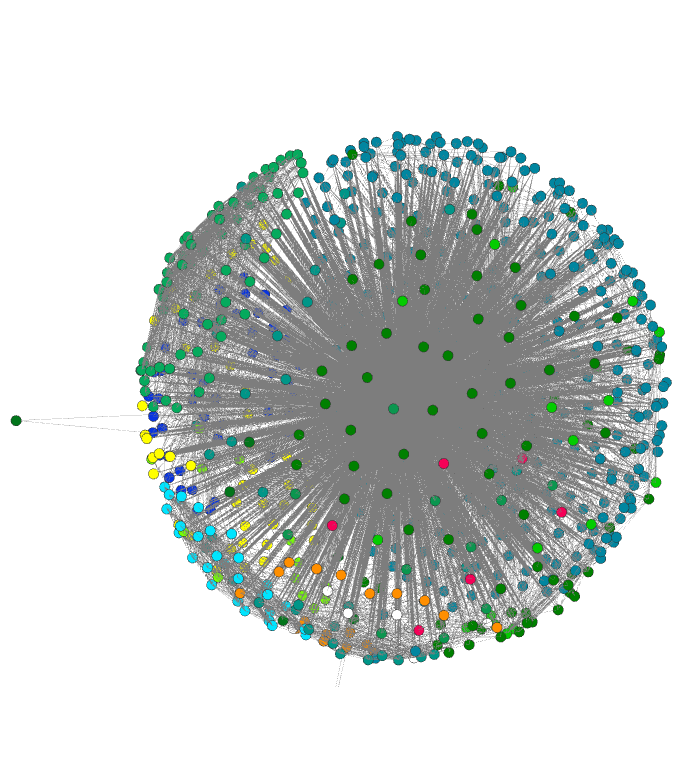
\includegraphics[width = 140mm]{nc_groundtruth.png}
	\caption{Grafo del sito \texttt{cs.illinois.edu}, etichettato manualmente.}
	\label{nc_graph}
\end{figure}
I grafi utilizzati rappresentano le due diverse operazioni di estrazione di collegamenti effettuate. La prima contiene tutti i collegamenti presenti all'interno di una pagina e mostrerà quindi più archi. La seconda estrae solamente gli hyperlink dalle liste.

\begin{table}[H]
	\begin{tabular}{| l | c | c | c | c | c |}
	\hline
	\textbf{Graph}  & \textbf{Homog} & \textbf{Compl} & \textbf{V-Measure}  & \textbf{ARI}  & \textbf{MI} \\ [3ex] \hline
	\textbf{nc WalkTrap} & 0.6471 & 0.6585 & 0.6527 & 0.4363 & 0.6281\\ [3ex]
	 \hline
	\textbf{nc Fastgreedy} & 0.5518 & 0.8563 & 0.6711 & 0.5764 & 0.5354\\ [3ex]
	 \hline	
	\textbf{lc WalkTrap} & 0.5093 & 0.4892 & 0.4991 & 0.2762 & 0.4722\\ [3ex]
	 \hline	
	\textbf{lc Fastgreedy} & 0.5522 & 0.6035 & 0.5767 & 0.3656 & 0.5382\\ [3ex]
	\hline
	\end{tabular}
	\caption{Risultati sperimentazione di partizionamento del grafo del sito \texttt{cs.illinois.edu}}
	\label{metricheGraph}
\end{table}

L'analisi del grafo considera unicamente le relazioni che intercorrono fra le pagine web e tralascia informazioni riguardanti il contenuto. Il grafo in figura \ref{nc_graph} rappresenta il sito web etichettato manualmente. Dalle metriche rilevate risulta in tabella \ref{metricheGraph}, risulta che il partizionamento del grafo web non riesce a dividere al meglio i cluster.


\subsection{URL Embedding}

Considerando i random walk generati sul grafo come frasi, è possibile applicare algoritmi di word embedding per raggruppare le pagine sulla base del contesto in cui appaiono, ovvero le pagine che più verosimilmente appariranno insieme nelle sequenze di random walk. Anche questo approccio considera unicamente le relazioni fra le pagine, ma of Apprendendo le rappresentazioni dai cammini, invece che dal partizionamento del grafo, è possibile codificare le pagine in uno spazio vettoriale con i benefici che conseguono. La fase di URL embedding è stata effetuata utilizzando l'algoritmo Word2vec.
\begin{figure}[h!]
	\centering
	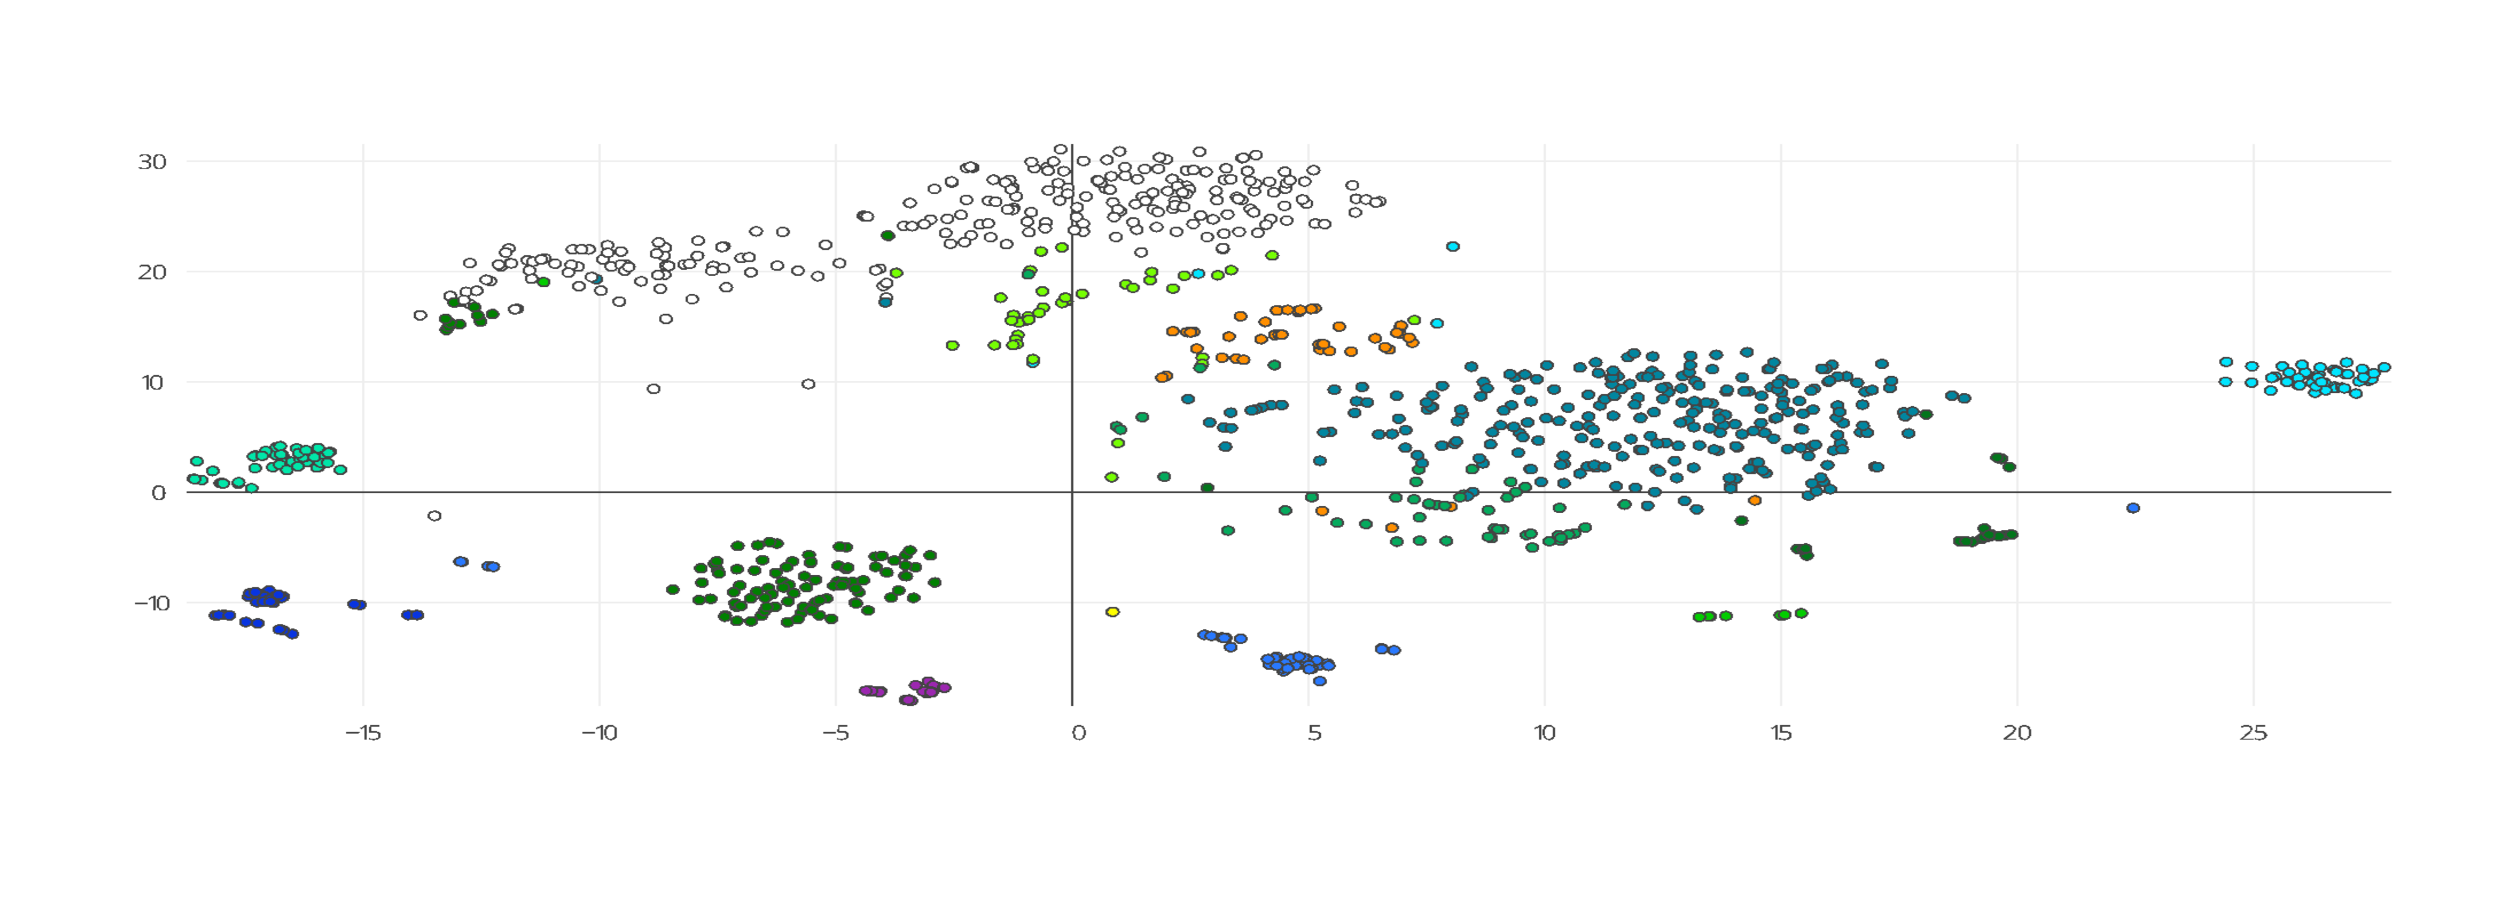
\includegraphics[width = 130mm]{lc_embedding_km.png}
	\caption{Rappresentazione del sito \texttt{cs.illinois.edu}, clusterizzato con K-Means.}
	\label{nc_embedding_km}
\end{figure}
\begin{table}[H]
	\begin{tabular}{| l | c | c | c | c | c | c |}
	\hline
	\textbf{Embed}  & \textbf{Homog} & \textbf{Compl} & \textbf{V-Meas}  & \textbf{ARI}  & \textbf{MI}  & \textbf{Silh} \\ [3ex] \hline
	\textbf{nc dbscan} & 0.5553 & 0.6579 & 0.6023 & 0.4487 & 0.5234 & 0.2588\\ [3ex]
	 \hline 
	\textbf{nc hdbscan} & 0.5759 & 0.6720 & 0.6203 & 0.5282 & 0.5525 & 0.2573\\ [3ex]
	 \hline
	\textbf{nc Kmeans} & 0.8238 & 0.7575 & 0.7892 & 0.7883 & 0.7423 & 0.3131\\ [3ex]
	 \hline	
	\textbf{lc dbscan} & 0.4163 & 0.5922 & 0.4889 & 0.2250 & 0.3935 & 0.1320\\ [3ex]
	\hline
	\textbf{lc hdbscan} & 0.4760 & 0.5067 & 0.4908 & 0.2275 & 0.4515 & 0.1054\\ [3ex]
	\hline
	
	\textbf{lc Kmeans} & 0.8095 & 0.6593 & 0.7267 & 0.6189 & 0.6473 & 0.2281\\ [3ex]
	\hline
	\end{tabular}
	\caption{Risultati sperimentazione di partizionamento del grafo del sito \texttt{cs.illinois.edu}}
	\label{metricheEmbed}
\end{table}

\subsection{Text Mining}
Qui viene effettuata l'analisi testuale della pagina web, utilizzando tecniche derivanti dal Text Mining. I contenuti all'interno di uno stesso sito web avranno una struttura e termini comuni, differenziandosi al variare dell'argomento trattato. La struttura gerarchica di un sito web organizza solitamente le pagine in sezioni simili. Questa metodologia tuttavia, considera solo l'informazione testuale, assumendo che i termini all'interno del sito web siano indipendenti l'uno dall'altro (cosa che nei documenti che trattano argomenti specifici non è vero) così come i documenti, ignorando le relazioni interdipendenti tra questi. Il web si discosta dall'analisi classica dei documenti proprio per le relazioni che intercorrono tra le pagine, tuttavia l'analisi testuale rimane molto importante.
\\
Nella fase di sperimentazione è stata utilizzata una rappresentazione vettoriale della frequenza dei termini all'interno dell'insieme delle pagine web, calcolata con la tecnica della \textit{frequency–inverse document frequency} (tf-idf).

\subsection{Informazione combinata}
I risultati hanno evidenziato che l'analisi singola, sia della correlazione tra le pagine sia del contenuto testuale, non basta a codificare esaustivamente la conoscenza che una pagina web può offrire. Entrambe le informazioni sono rilevanti ed andrebbero processate combinatamente. Il vantaggio di associare le relazioni in uno spazio vettoriale offre il vantaggio usare la stessa rappresentazione e quindi di unire i vettori derivanti dagli algoritmi di word embedding con quelli derivanti dall'analisi di contenuto testuale. 
\\
Così facendo è possibile dare più importanza ad una tipologia di informazione piuttosto che ad un altra, andando a modificare il rapporto tra le dimensioni dei vettori.






\chapter{Conclusioni e sviluppi futuri}
% !TEX encoding = UTF-8
% !TEX TS-program = pdflatex
% !TEX root = ../Tesi.tex
% !TEX spellcheck = it-IT

%*******************************************************
% Introduzione
%*******************************************************
In questo lavoro di tesi è stato trattato il clustering di pagine Web, proponendo una nuova metodologia.
La trattazione effettuata è incentrata sull'utilizzo dei Random Walk per apprendere rappresentazioni vettoriali delle pagine, unitamente al loro contenuto testuale. Il lavoro non pretende di essere esaustivo, ma piuttosto un punto di partenza per ulteriori sviluppi, sia teorici che sperimentali. 
\\\\
I risultati sperimentali prodotti si sono rivelati discreti e incentivano a proseguire gli studi in questa direzione in modo da individuare nuove tecniche che permettano di migliorare i risultati raggiunti in termini di qualità. 
In particolare è stato osservato come la forma dei cluster vari in funzione dal Dataset. Quindi, sarebbe opportuno utilizzare l'algoritmo più appropriato in base al contesto. 
\\
Da notare come le ''analogie'' estraibili dall'utilizzo di \textit{Word2vec} su collezioni di documenti, abbiano avuto un riscontro nel Web.

%% !TEX encoding = UTF-8
% !TEX TS-program = pdflatex
% !TEX root = ../Tesi.tex
% !TEX spellcheck = it-IT

%************************************************
\chapter{Ipsum}
\label{cap:ipsum}
%************************************************


Lorem ipsum dolor sit amet, consectetuer adipiscing elit. Nam dui ligula, fringilla a, euismod sodales, sollicitudin vel, wisi. Morbi auctor lorem non justo. Nam lacus libero, pretium at, lobortis vitae, ultricies et, tellus.
\begin{description}
\item[Lorem ipsum dolor] sit amet, consectetuer adipiscing elit. Ut purus elit, vestibulum ut, placerat ac $\lim_{n \to \infty}\sum_{k=1}^n \frac{1}{k^2}= \frac{\pi^2}{6}$.
\item[Mauris ut leo.]
Cras viverra metus rhoncus sem. Nulla et lectus vestibulum urna fringilla ultrices. Phasellus eu tellus sit amet tortor gravida placerat.
\[
\lim_{n \to \infty}\sum_{k=1}^n \frac{1}{k^2}= \frac{\pi^2}{6}.
\]
\end{description}

Nulla malesuada porttitor diam. Donec felis erat, congue non, volutpat at, tincidunt tristique, libero. Vivamus viverra fermentum felis.
\begin{equation}
\label{eq:euler}
e^{i\pi}+1=0.
\end{equation}
Dalla formula~\eqref{eq:euler} 
si deduce che\dots






\section{Nozioni basilari}

\subsection{Insiemi numerici}

Donec nonummy pellentesque ante. Phasellus adipiscing semper elit.
\begin{equation}
x^2 \geq 0 \quad
\forall x \in \mathbb{R}.
\end{equation}


\subsection{Le matrici}

\lipsum[2]
\begin{equation}
A=
\begin{bmatrix}
x_{11} & x_{12} & \dots \\
x_{21} & x_{22} & \dots \\
\vdots & \vdots & \ddots
\end{bmatrix}
\end{equation}



\section{Formule fuori corpo}

Proin fermentum massa ac quam. Sed diam turpis, molestie vitae, placerat a, molestie nec, leo. Maecenas lacinia. Nam ipsum ligula, eleifend at, accumsan nec, suscipit a, ipsum. 


\subsection{Una formula spezzata con allineamento}

\lipsum[2]
\begin{equation} 
\begin{split} 
a &= b+c-d \\ 
  &= e-f \\ 
  &= g+h \\ 
  &= i. 
\end{split} 
\end{equation}

 
\subsection{Casi}

\lipsum[3]
\begin{equation}
f(n):=
\begin{cases} 
2n+1, & \text{con $n$ dispari,} \\ 
n/2,  & \text{con $n$ pari.} 
\end{cases} 
\end{equation}



\section{Enunciati e dimostrazioni}

Nunc eleifend consequat lorem. Sed lacinia nulla vitae enim. Pellentesque tincidunt purus vel magna. Integer non enim. Praesent euismod nunc eu purus.
\begin{definizione}[di Gauss] 
Un \emph{matematico} trova ovvio che
$\int_{-\infty}^{+\infty}
e^{-x^2}\,dx=\sqrt{\pi}$. 
\end{definizione} 
\begin{teorema} 
I matematici, se ce ne sono, sono molto rari.
\end{teorema} 

\lipsum[2]

\begin{teorema}[di Pitagora]
La somma dei quadrati costruiti sui cateti uguaglia il quadrato costruito sull'ipotenusa.
\end{teorema}
La dimostrazione viene lasciata per esercizio.

Donec bibendum quam in tellus. Nullam cursus pulvinar lectus. Donec et mi. Nam vulputate metus eu enim. Vestibulum pellentesque felis eu massa.
\begin{teorema}[Sorpresa]
Si ha che $\log(-1)^2=2\log(-1)$.
\end{teorema} 
\begin{proof} 
Si ha che $\log(1)^2 = 2\log(1)$.
Ma si ha anche che $\log(-1)^2=\log(1)=0$.
Quindi $2\log(-1)=0$, da cui la tesi.
\end{proof}
Viene un quadratino a fine dimostrazione.
\begin{legge}
\label{lex:capo}
Il capo ha ragione.
\end{legge}
\begin{decreto}[Aggiornamento alla legge~\ref{lex:capo}]
Il capo ha \emph{sempre} ragione.
\end{decreto}
\begin{legge}
Se il capo ha torto, vedere la 
legge~\ref{lex:capo}.
\end{legge}


Nam dui ligula, fringilla a, euismod sodales, sollicitudin vel, wisi. Morbi auctor lorem non justo. Nam lacus libero, pretium at, lobortis vitae, ultricies et, tellus.
\begin{murphy}
Cras nec ante. Pellentesque a nulla. Cum sociis natoque penatibus et magnis dis parturient montes, nascetur ridiculus mus. Aliquam tincidunt urna.
\end{murphy}

%\appendix
%\input{Capitoli/Dolor}
% *****************************************************************
% Materiale finale
%******************************************************************
%% !TEX encoding = UTF-8
% !TEX TS-program = pdflatex
% !TEX root = ../Tesi.tex
% !TEX spellcheck = it-IT

%*******************************************************
% Introduzione
%*******************************************************
In questo lavoro di tesi è stato trattato il clustering di pagine Web, proponendo una nuova metodologia.
La trattazione effettuata è incentrata sull'utilizzo dei Random Walk per apprendere rappresentazioni vettoriali delle pagine, unitamente al loro contenuto testuale. Il lavoro non pretende di essere esaustivo, ma piuttosto un punto di partenza per ulteriori sviluppi, sia teorici che sperimentali. 
\\\\
I risultati sperimentali prodotti si sono rivelati discreti e incentivano a proseguire gli studi in questa direzione in modo da individuare nuove tecniche che permettano di migliorare i risultati raggiunti in termini di qualità. 
In particolare è stato osservato come la forma dei cluster vari in funzione dal Dataset. Quindi, sarebbe opportuno utilizzare l'algoritmo più appropriato in base al contesto. 
\\
Da notare come le ''analogie'' estraibili dall'utilizzo di \textit{Word2vec} su collezioni di documenti, abbiano avuto un riscontro nel Web.
\bibliographystyle{plain}
\bibliography{Bibliografia}                % database di biblatex 

\end{document}
